

\documentclass[journal,transmag]{IEEEtran}


% *** GRAPHICS RELATED PACKAGES ***
%
\ifCLASSINFOpdf

\else

\fi




% correct bad hyphenation here
\usepackage{booktabs} % For formal tables
\usepackage{indentfirst} % For formal tables\cite{}
\usepackage{url} % For formal tables
\usepackage{graphicx}
\usepackage{balance}  % for  \balance command ON LAST PAGE  (only there!)
\usepackage{caption}
\usepackage{subfig}
\usepackage{amsmath}
\usepackage{amssymb}
\usepackage{algorithm}
%\usepackage{algorithmic}
\usepackage{color}
\usepackage{comment}
\usepackage{flushend}
\usepackage{bm}
\usepackage{algpseudocode}
\usepackage{amsthm}

\renewcommand{\algorithmicrequire}{\textbf{Input:}}
\renewcommand{\algorithmicensure}{\textbf{Output:}}
\newtheorem{theorem}{Theorem}
\hyphenation{op-tical net-works semi-conduc-tor}
\newcommand{\Paragraph}[1]{\smallskip{\bf #1.}}

\begin{document}

\title{PowerHash: A Hash Grouping Scheme by Leveraging Power-Law Properties of Data}
%\IEEEauthorrefmark{2}
\author{\IEEEauthorblockN{Xun Wei, \textcolor{red}{Xiaowang Kong}, Yanfeng Zhang, Ge Yu}
Northeastern University, Liaoning, 110819, China
\IEEEauthorblockN{1670851@stu.neu.edu.com, {zhangyf,yuge}@mail.neu.edu.cn}
}








\IEEEtitleabstractindextext{%
\begin{abstract}
%We study the GroupBy implementation found in MapReduce and databases. GroupBy operation partitions a set of records into groups according to some key. Despite its  wide range of applications, most existing GroupBy implementations become very inefficient when the input data are too large to be hold in main memory, if the group sizes of input data follow the power-law distributions, their performances will be worse because of a large amount of repeat access to disk caused by distribution unbalance. We propose an I/O efficient GroupBy implementation \emph{Power-Law Hash} that leverages the features of power-law distributions. In order to reduce the I/O cost in GroupBy operation with limited memory, power-law hash copes with the big groups and small groups separately by indexing-filling and partitioned hash approach. We put forward to divide the big groups and small groups by the count-min sketch and Pareto principle. Given the same memory resource budget, power-law hash improves the execution time a lot compared with some existing GroupBy implementations.
We study the GroupBy implementation scheme widely used in distributed systems and databases. The GroupBy operation partitions a set of out-of-order records into groups. Due to the massive data size, many I/O efficient grouping schemes that exploit external memory have been proposed. In this paper, we observe that the group sizes of input data exhibit power-law property and the grouping schemes' performance varies a lot for data with different group sizes. The \emph{indexing-filling} approach prefers data with big group size, while the \emph{partitioned hash} approach prefers data with small group size. Based on this observation, we propose a hybrid approach, \emph{PowerHash}, which invokes different grouping schemes for different data. The group size information is approximately estimated by the count-min sketch so that the big groups and small groups can be distinguished from each other. With a given memory budget, our results show that PowerHash can improve the performance by \textcolor{red}{25\%-100\%} times over the existing GroupBy implementations.


\end{abstract}

% Note that keywords are not normally used for peerreview papers.
\begin{IEEEkeywords}
key value grouping, power-law distribution, GroupBy, hashtable.
\end{IEEEkeywords}}



% make the title area
\maketitle

\IEEEdisplaynontitleabstractindextext

\IEEEpeerreviewmaketitle


\section{Introduction}

Key value grouping operation, known as GROUP BY clause, is a key operation in database systems \cite{gray1997data}, \cite{stephens2005oracle}, \cite{mysql2009mysql}, \cite{momjian2001postgresql}. It groups a set of out-of-order records into multiple groups according to a certain key. GroupBy operation is often used with aggregate functions which produces a single row of summary information for each group, e.g., GroupBy-Aggregate in SQL. GroupBy is also widely used in distributed computing frameworks for distributing and locating the data. MapReduce \cite{dean2008mapreduce} expresses the computational process as three phases: Map, Shuffle and Reduce. During the shuffle phase, the key-value pairs that have the same key are aggregated together to form a Map output file, and they are sent to the same Reduce processor where the final cluster-wide aggregation (reduction) is applied on them. The efficiency of the key-value grouping step is crucial to both relational databases and distributed computing systems.


%Another popular use case for key grouping is to accumulate state across the stream in distributed stream processing engines (DSPEs) such as Storm \cite{storm2013storm}, S4 \cite{neumeyer2010s4}, Smaza \cite{noghabi2017samza}. This grouping in DSPEs is usually implemented by partitioning the stream on a key \cite{nasir2015power}. The strategies that are used to route tuples in a stream toward available operators can be divided into two categories: key grouping for stateful operators where a stream of tuples is partitioned in several disjoint sub-streams depending on the values contained \cite{rivetti2015efficient} and shuffle grouping for stateless operators where each tuple of a stream can be randomly assigned to any available operator \cite{Rivetti2016Online}. However, all the above works are focused on how to route kv-pairs to available operators for alleviating load imbalance but ignoring local key value aggregation overhead at the receiver side. In fact, the execution time depends on not only stream partition but also local aggregation. Our work will focus on accelerating the local GroupBy aggregation in this paper.

There are two categories of GroupBy implementations in general, sort-based grouping and hash-based grouping. Basically, the \emph{sort-based grouping} makes the data records sorted in the order of the group key, so that the records with the same group key are located together. While the \emph{hash-based grouping} typically hashes key-value pairs to a hash table structure where multiple key-value pairs in the same group (sharing the same group key) are stored in the same bucket.

Recall that key-value pairs (kv-pairs) grouping operation is the key operation in Hadoop MapReduce \cite{dean2008mapreduce}. The map output kv-pairs are locally grouped by keys before they are shuffled to reduce workers. These map output kv-pairs (i.e., reduce input kv-pairs) from various map workers are further merged to obtain a global grouped kv-pairs. Each group of kv-pairs sharing the same key is the input of a reduce function. In Hadoop Mapreduce implementation, a kind of sort-based grouping, \emph{merge-sort grouping}, is used, which can perform quite general grouping tasks at scale even in the absence of available memory. However, merge-sort grouping involves large amount of redundant computation and I/Os. The previous work \cite{shvachko2010hadoop,yu2009distributed,Li2011A} shows that merge-sort grouping adopted by Hadoop is found to be among the worst-performing choices.

For many applications, hash-based grouping is adopted because these applications require only unsorted grouping \cite{lin2011tenzing}, \cite{yu2009distributed}. However, hash-based grouping consumes more memory than sort-based grouping because it requires to load all records into memory. The performance heavily depends on the amount of available memory. A variant of hash grouping has been used in MariaDB \cite{bartholomew2012mariadb}, Oracle \cite{stephens2005oracle}, Postgresql \cite{momjian2001postgresql}, and SQL Server \cite{agrawal2005database}. It creates an in-memory hash table for grouping rows. If the hash table becomes too large to be fit in memory, the input records are partitioned into smaller work tables which are recursively partitioned until they fit into memory. Once all input groups have been processed, the completed in-memory groups are output and repeat the algorithm by reading back and aggregating one spilled partition at a time until all partitions have been processed. We refer to this approach as \emph{memory-constraint hash grouping}. It excels at efficiently aggregating large data sets and performs better than merge-sort grouping in some situations.

An alternate of hash grouping that can avoid memory overflow is using rehashing. The first hash grouping is applied to obtain coarse-grain kv-pair groups, where each group of kv-pairs covering multiple unique keys is written to a disk file. The second phase loads each kv-pairs file into memory and performs hash grouping on keys, so that the kv-pairs sharing the same key are grouped together in a bucket. These grouped kv-pairs are then written out for recycling memory to group next coarse-grain grouped kv-pairs (in next file). The number of files (coarse-grain groups) can be tuned according to available memory, and further optimizations can be applied to avoid memory overflow when processing each coarse-grain group. We refer to this approach as \emph{partitioned hash grouping}.

In addition, we can use an \emph{indexing-filling} approach that takes advantages from both sort grouping and hash grouping. A nice property of sort-based grouping is that the output file position of each group is determined before the grouping starts. While in hash-based grouping, the query of a specific group can be very fast. It first reads all data in one pass and evaluates the group size information associated for each key, which is maintained in an in-memory table. The output file offsets of all groups can be then calculated. In other words, the output kv-pairs are indexed in the first indexing phase. Then the data are parsed for the second time, and the kv-pairs are written out to specific file positions according to the offset table, which is the filling phase. Note that, the write operations can be cached to be sequential for I/O efficiency.

\begin{figure}[t]%figure 2
\subfloat[Performance comparison on big groups]{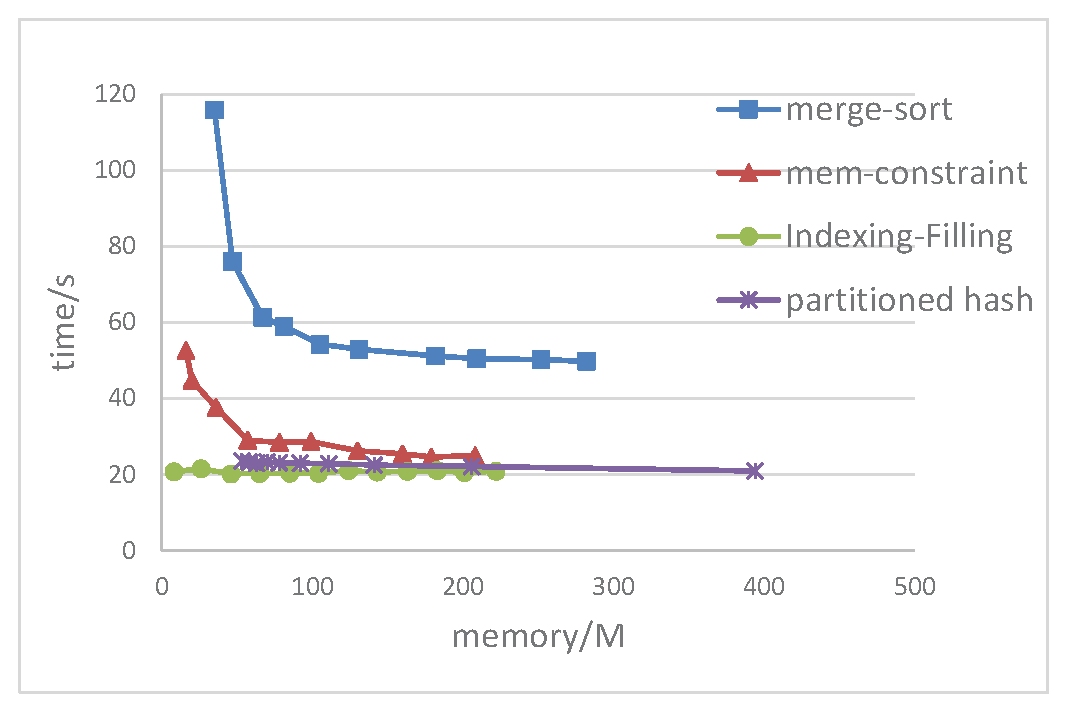
\includegraphics[width = 1.68in]{fig/paretoBig.eps}\label{fig:paretoBig}}
    \hspace{0.23cm}
    \subfloat[Performance comparison on small groups]{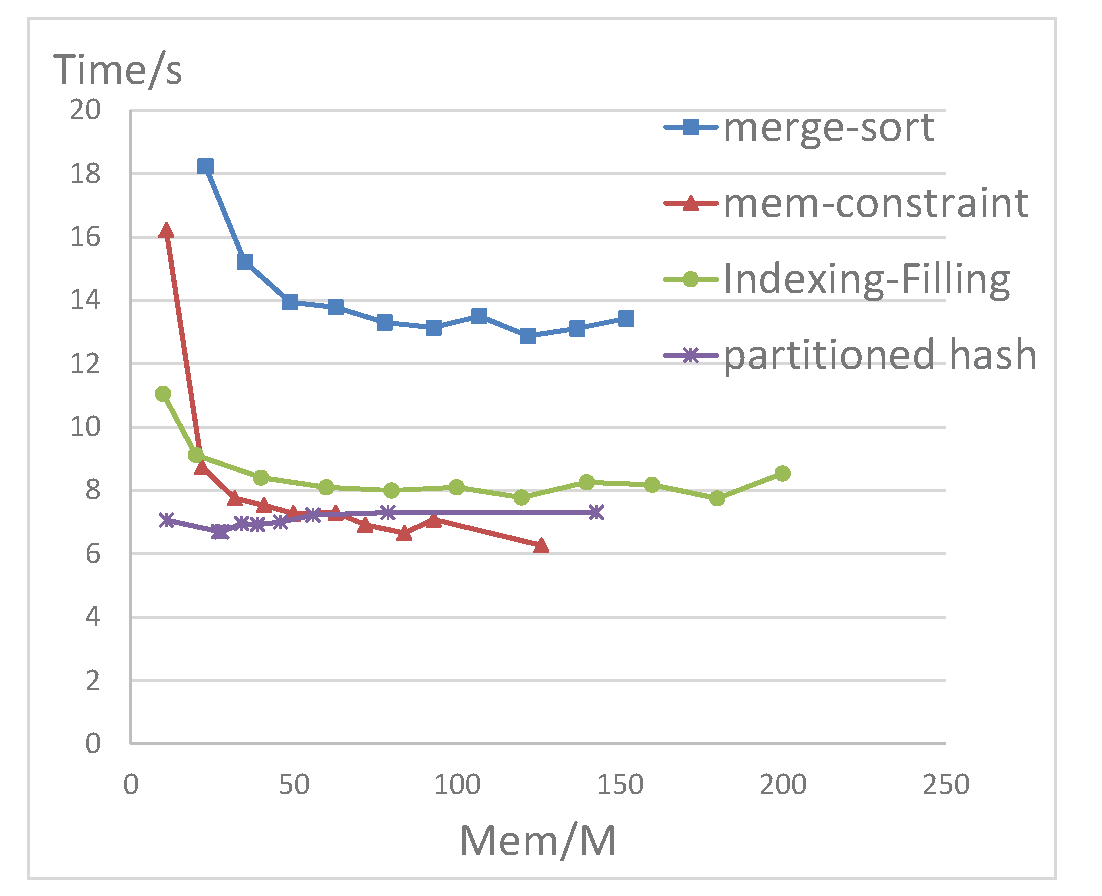
\includegraphics[width =1.68in]{fig/paretoSmall.eps}\label{fig:paretoSmall}}\\
%\includegraphics[width=.5\textwidth]{fig/pareto_index_hash}
\caption{Performance comparison of big groups and small groups. The big groups and small groups are extracted from a simulation data set Pareto, the group sizes of Pareto follow a power-law distribution.}
\label{fig: big and small}
\end{figure}

After reviewing these grouping algorithms, one question is raised. Which one is the best? Our results show that no one wins all the time. As known, the group sizes in real data sets follow power-law distributions, the big group sizes and small group sizes vary over an enormous range. We further observe that these implementations exhibit different performance and memory usage for big groups and small groups. We extract the kv-pairs of big groups and small groups from Pareto dataset respectively and evaluate the above four algorithms on grouping time and memory usage. For any method, using more memory will group data faster, so we show the results with both memory cost and runtime. With the same memory budget, the shorter runtime the better. The result for grouping big groups is shown in Figure \ref{fig:paretoBig}, where the \emph{indexing and filling} method performs the best over the others. The reason is that filling the output files with big groups will lead to relatively large amount of sequential writes but less number of seeks, which is good for I/O efficiency. On the other hand, the partitioned hash and the memory-constraint hash outperform the others for grouping small groups as shown in Figure \ref{fig:paretoSmall}. Considering the extremely large input size, we would like to compare them with limited memory. The partitioned hash grouping runs faster with limited memory.


%When these data sets are processed by memory-constrain hash grouping in limited memory, the sub-tables sizes are not balanced caused by big groups, which leads to multiple recursive partitions and downgrade grouping performance. The performance reduction resulting from power-law distributions often occurs in various applications, we observe that these implementations exhibit different performance and memory usage for big groups and small groups. As shown in Figure \ref{fig:paretoBig}, the \emph{indexing and filling} method performs the best when grouping the big groups. Indexing and filling method proposed in this article is a file filling process according to an index, it creates an in-memory offset index which records each group's output position in result file firstly and fills the result file on the basis of the offset index, so the best grouping approach is indexing and filling for big groups. As shown in Figure \ref{fig:paretoSmall}, the \emph{partitioned hash grouping} method runs faster in limited memory when grouping small groups, that the kv-pairs in small groups are processed partition by partition is refered as partitioned hash grouping, so grouping small groups by partitioned hash is the best choice. Therefore, the ideal implementation should take the group size into account, and a hybrid grouping approach is desired.




Based on this observation, we propose an I/O efficient hash grouping scheme \emph{PowerHash} that leverages power-law property of the data group sizes. The big groups and small groups are processed separately. The kv-pairs of big groups are grouped by indexing-filling method, and the kv-pairs of small groups are grouped by the partitioned hash grouping approach. However there are two problems raised, how to estimate the group sizes efficiently and how to distinguish between the big groups and small groups? We solve the first problem by using the count-min sketch \cite{Cormode2009Count} to approximately estimate the group sizes. We formalize the second problem as an optimization problem and obtain the boundary of big and small groups given a memory budget. Our experimental results show that PowerHash always outperforms the other counterparts on real datasets. With the same memory cost, PowerHash is \textcolor{red}{25\%-100\%} times faster than the merge-sort grouping and at least \textcolor{red}{100\%-200\%} times faster than the memory-constraint hash grouping.

%The whole process of key grouping by power-law hash can avoid unnecessary repeat access to disk and needs less memory. When dealing with the big groups, the kv-pairs in big groups are written to the result file directly on the basis of offset index, only the offset index is stored in memory during the grouping process of big groups, the offset index size is much less than the big groups sizes and there is no need to load any whole group into memory, so the writing back to disk caused by out-of-memory can be prevented and the I/O cost can be reduced. For a data set whose group sizes follow a power-law distribution, the majority of the data set has been written to the result file after dealing with the big groups. So partition unbalance can be avoided to a great extent because there is no big groups in the remaining data set when we partition the small groups, and then it can prevent multiple recursive division to the big partitions.

%Our main contributions can be summarized as follows:
\begin{comment}
\begin{list}{\labelitemi}{\setlength{\leftmargin}{5mm}\setlength{\itemindent}{0mm}
\setlength{\topsep}{0.5mm}\setlength{\itemsep}{2mm}\setlength{\parsep}{0mm}}
\item Firstly, we study the problem of key grouping in modern distributed processing engines and traditional relation databases.
\item Secondly, we present an I/O efficient hash grouping scheme that leverages the power-law distributions and hashing, which can complete the key grouping operation with less memory usage and time cost.
\item Thirdly, we evaluate our algorithm through extensive experiments. The results show that power-law hash improves the performance with the same limited memory usage compared to memory-constraint hash, the runntime gap is greater compared to merge-sort.
\end{list}
\end{comment}

The rest of this paper is organized as follows. Section \uppercase\expandafter{\romannumeral2} describes the related work. In Section \uppercase\expandafter{\romannumeral3}, we propose our grouping method power-law hash and present the key optimizations. Section \uppercase\expandafter{\romannumeral4} discusses the parameters setting. The experimental results are presented in Section \uppercase\expandafter{\romannumeral5}. Finally, Section \uppercase\expandafter{\romannumeral6} concludes the paper.


\section{Related Work}
\label{sec:related}

% A increasingly large body of work has focused on the problem of key grouping (or Group By). There are two categories of GroupBy implementations in general, sort-based grouping and hash-based grouping. Each of these algorithms can be used for anywhere in database query related to grouping (Group By, SUM, AVE, etc) \cite{Hellerstein1996Query}.
This section provides some backgrounds on existing key grouping approaches and reviews the count-min sketch that will be used in our algorithm.
%Section A introduces the merge-sort grouping algorithm and Section B provides a detailed description on memory-constraint hash algorithm for SQL Hash GroupBy clause,  Section C and D introduces the power-law distributions  and the count-min sketch.

\subsection{Commonly Used Grouping Implementations}%2.1

\Paragraph{Merge-Sort Grouping} One of the most widely used grouping algorithm is merge-sort grouping, which is widely used in MapReduce \cite{dean2008mapreduce} and SQL Group By operator \cite{nasir2015power},\cite{mysql2009mysql},\cite{boicea2012mongodb},\cite{momjian2001postgresql},\cite{agrawal2005database}. The Hadoop MapReduce uses a merge-sort at both the Map and Reduce phases to group kv-pairs. These kv-pairs to be grouped will be constantly written to the memory buffer. The buffer is used to collect kv-pairs in batches, so as to minimize the impact of disk I/O. The entire buffer size is limited. As the amount of data in the buffer reaches the threshold, a background spilled thread sorts these kv-pairs in the memory buffer in accordance with the key, and writes these kv-pairs that have been sorted in the buffer to disk as a partial sorted file. Each spilling operation generates a spilled file on disk. Finally, a merge phase is required to sort these partial sorted files to generate the final sorted file (i.e., the data in the file are grouped). Merge-sort can achieve the purpose of aggregating kv-pairs for any amount of data, which is highly scalable. However, keeping different groups in order is unnecessary because the aim is making the kv-pairs that are in the same key continuously stored on disk. Therefore, merge-sort grouping will result in unnecessary computational overhead.


%In SQL database, The default Group By implementation is to scan the entire table, e.g. group records in table by merge-sort algorithm or make use of index based on columns specified by Group By clause to avoid sorting again \cite{mysql2009mysql}. Sorting is never  the  best, except  when  tables  are ordered  in  advance  or  when the  result  have  to  be sorted  on operation  key \cite{Bratbergsengen1984Hashing}.


%However, the execution efficiency is not high enough. The merge-sort algorithm aggregates kv-pairs with the same key by sorting key completely, so that the grouping keys are ordered among different groups. Commonly, keeping different groups in order is redundant because the aim of grouping is to store kv-pairs having the same key on adjacent locations on the disk, and it��s irrelevant Whether grouping keys are sorted between two groups. Therefore, merge-sort for aggregating kv-pairs will result in unnecessary computational overhead. on the other hand, the amount of memory required for sorting is proportional to the total number of kv-pairs in the buffer rather than the number of distinct keys.


\Paragraph{Memory-Constraint Hash Grouping}%2.2
Some SQL databases (e.g., MariaDB) that use a hash grouping aggregation strategy for GroupBy operations \cite{bartholomew2012mariadb}. We refer to this approach as \emph{memory-constraint hash grouping}.  The memory-constraint hash is similar to hash join, it does not require sort but more memory. \textcolor{red}{Memory-constraint hash partitions the large task  into smaller subtasks  where the subtasks can be executed in memory completely \cite{Bratbergsengen1984Hashing},\cite{HashAggregate15}. If the size of data to be grouped exceeds the memory limit, one or more buckets will be spilled to disk. Then the records that are hashed to the spilled buckets will be divided up into the corresponding partitions in disk. Once all input groups have been processed, the completed in-memory groups will be output and repeat the algorithm by reading back and aggregating one spilled partition at a time. However, when processing data sets whose group sizes follow power-law distributions, the sub-tables sizes are not balanced, which leads to multiple recursive partitions and downgrade grouping performance.}

%including any partial aggregated results along with any additional new rows that will be hashed to the spilled buckets or partitions


\subsection{Group Size Distribution}
%Many of the things that scientists measure have a typical size or ``scale'' --- a typical value around which individual measurements are centred. But not all things we measure are peaked around a typical value, some vary over an enormous dynamic range \cite{MEJPower}, those things following the power-law distributions are like this.

\textcolor{red}{should be rewrite, please refer to PowerGraph paper. The goal is to tell readers the group sizes are indeed following powerlaw distribution. Besides the figure, you might want to show some numbers, like 99\% data are from top 10\% big groups, or some thing like that. You might also want to say some thing that for the extremely large groups, the traditional grouping tech will not work. and say why}

%Power-law distributions occur in an extraordinarily diverse range of phenomena, e.g., the frequency of use of words in any human language \cite{George1949Human}, the number of hits on web pages \cite{Adamic2000The}. Those things following the power-law distributions are always right-skewed, it means that a bulk of the distribution occurs for fairly small sizes and only a small number of data in it are much higher than the typical value. When we carry out key grouping operation, the group sizes in many real data sets follow the power-law distributions as shown in Figure \ref{fig: distributions}.

\begin{figure}[t]%figure 2
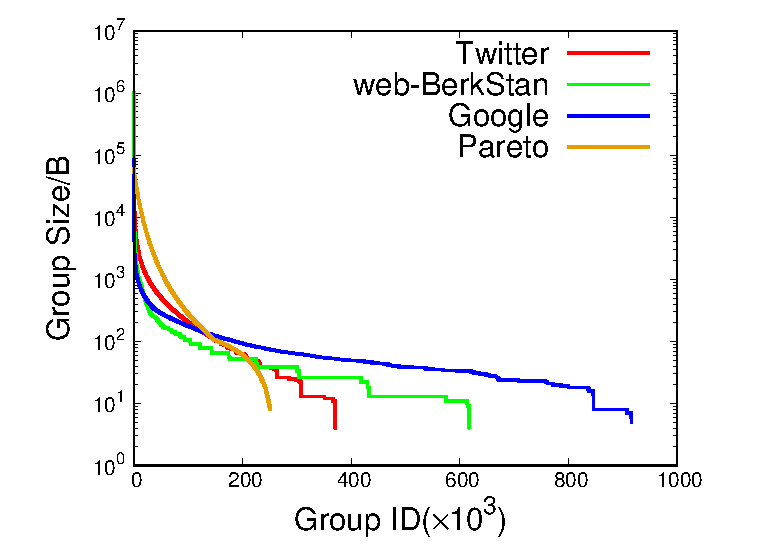
\includegraphics[width = 2.8in]{fig/distributions.eps}
%\includegraphics[width=.5\textwidth]{fig/pareto_index_hash}
\caption{The group sizes distributions for different datasets.}
\label{fig: distributions}
\end{figure}


%Based on the right-skew property of power-law distributions in reality, Pareto principle(also known as 80/20 rule)\cite{Box1986An}, \cite{MEJPower} is proposed, it is is borne out by more detailed observations of the wealth distribution. It states that about 80\% of the wealth should be in the hands of the richest 20\% of the population(the so-called ``80/20 rule''). According to the Pareto principle, we can get that roughly 80\% of the effects come from 20\% of the causes for many events. Mathematically, the 80/20 rule is roughly followed by a power-law distribution for a particular set of parameters. Besides the wealth distribution, the Pareto principle can be applied to optimization efforts in computer science, engineering control\cite{Gen2000Network} and many other applications.

%For a data set whose group sizes follow a power-law distribution, we can distinguish between the big groups and small groups roughly on the basis the Pareto principle, the ratio between big groups and small groups obeys the 80/20 rule.
%We extract the groups that are the top 20\% in size from four data sets, these big groups occupy about 80\% of the data sets as shown in Table \ref{tab:percentage}.

\begin{comment}
\begin{table}
  \caption{Percentage of the size of the big groups}
  \label{tab:percentage}
  \begin{tabular}{cccc}
    \toprule
    dataset & total size & big group size & percentage\\
    \midrule
    Twitter & 180.4MB & 142MB & 78\%\\	
	web-BerkStan & 102.5MB & 80.0MB &78\%\\
	Google & 97.2MB & 61M & 63\%
	Pareto  & 575.4MB & 519MB & 90\%\\
    \bottomrule
  \end{tabular}
\end{table}
\end{comment}


\subsection{The Count-Min Sketch}

The count-min sketch (CM sketch)\cite{Cormode2009Count},\cite{10.1007/978-3-540-24698-5_7} is a probabilistic data structure that serves as a frequency table of events in a data stream, it uses hash functions to map events to frequencies at the expense of overcounting some events due to collisions.
%A count-min sketch typically has a sublinear number of cells, related to the desired approximation quality of the sketch. \
%If the error of group sizes is within a factor of $ \varepsilon $ with probability $ \delta$, the depth $d$ is $\lceil ln(1/\delta) \rceil $, the width $w$ is $\lceil e/\varepsilon\rceil $. Each entry of the array is initially zero.

A CM sketch is represented by a two-dimensional array counting with width $w$ and depth $d$. Additionally, $d$ hash functions $h_{1} ...h_{d}$ are chosen uniformly at random from a pairwise-independent family. The space used by Count-Min sketches is the two-dimensional array and $d$ hash functions. The CM sketch is simple to construct and counting the frequencies of the unique items in data stream quickly.

%In our algorithm, the CM sketch will be used to counting the group sizes in the data sets, the distinction between big groups and small groups is based on these rough group sizes. When calculating the group sizes, the CM sketch has the two basic operations: counting first and computing the minimum next.

\textcolor{red}{the following paragraphs should be rewriten, what is $h_j$? Also, please give more intuitions.}

We first traverse the input data set to be grouped, when getting a $\langle key, value\rangle$ pair, meaning that this kv-pair belongs to a group with unique $key$, the group size will be updated by the kv-pair size $sizeof(kv)$, then $sizeof(kv)$ are added to one count in each row; the counter is determined by $h_{j}$. Formally, set $\forall 1 \leq j \leq d: count[j,h_{j}(key)]\leftarrow count[j,h_{j}(key)] + sizeof(kv)$. After traversing, the size to a group with $key$ is given by $f_{key} = min_{j}count[j,h_{j}(key)]$.

On the other hand, each row of the CM sketch can reflect the distribution of group sizes, this property can help us distinguish the big groups and small groups with avoiding large-scale sorting.



Our strategy is to leverage the CM sketch to counting the group sizes in the data set roughly, the rough group sizes are used to distinguish between the big groups and small groups depending on Pareto principle. Then the big groups and small groups are processed separately, the big groups are grouped by the indexing and filling method to reduce the I/O cost, the small groups are processed by partitioned hash grouping approach. PowerHash can finish the key grouping operation in limited memory with high efficiency.

\section{Power-Law Hash Design and Implementation}
\label{sec:hash}

In key grouping operation, many grouping approaches need to spill part of kv-pairs to disk when the memory used has reached the threshold, these spilled partitions will be read back to re-aggregate subsequently. If the group sizes of data set follow a power-law distribution, 
it is more difficult for these approaches to divide the work data into small uniform portions, then several great partitions may be create if some big groups are spilled to the same portion. For a large partition spilled to disk, subsequent reading back and re-aggregating may lead to recursively execute the process many times when the memory is limited, the I/O overhead increases sharply. So we take the group size into account and propose to deal with the big groups and small groups separately. And we found that the indexing and filling method is suitable for big group key grouping, and the partitioned hash grouping is a good choice for small groups. For the data sets whose group sizes follow power-law distributions, the total size of big groups occupies the majority of the data sets but the number of big groups is minority, these properties of small groups are just the opposite, so this idea of processing separately is applicable for these data set and the powerhash algorithm is proposed. 

\subsection{Overview of Powerhash}%3.1
Depending on the core idea of power-law hash, our algorithm can be divided into three phases: Distinguishing, Indexing and Filling, Partitioned hash. The whole process is shown in Figure \ref{fig:pwHash}.
\begin{figure}
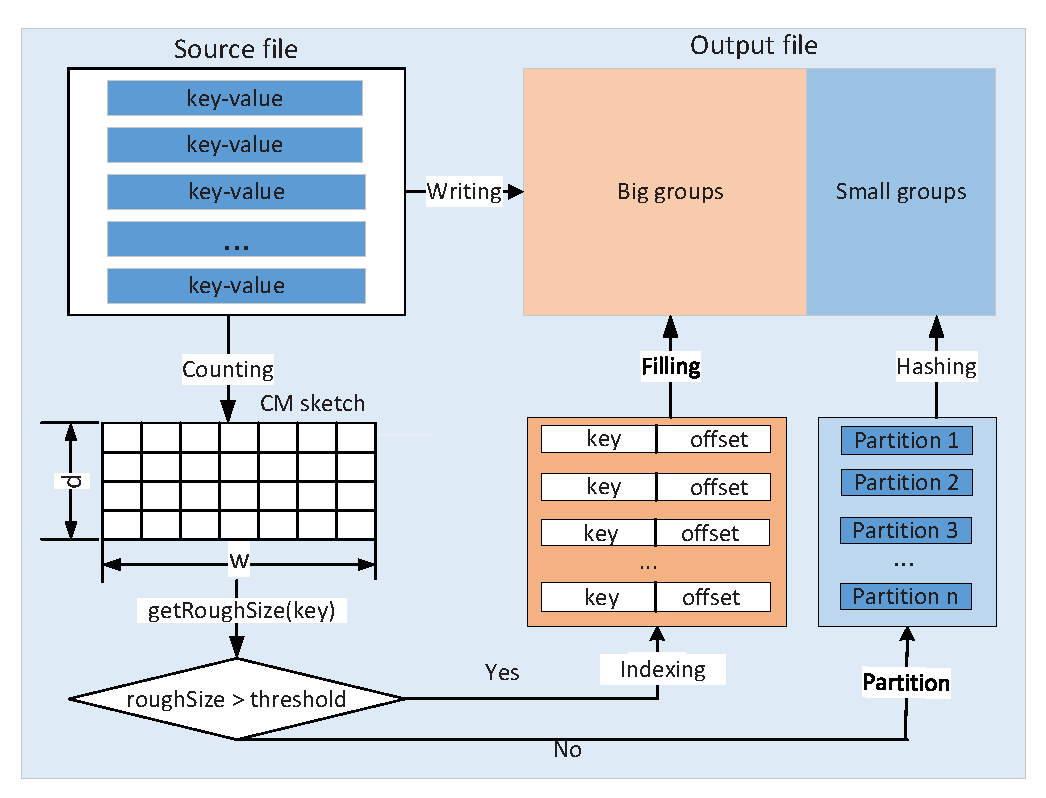
\includegraphics[width=.5\textwidth]{fig/pwhash}
\caption{Overview Intuition of Power-Law Hash.}
\label{fig:pwHash}
\end{figure}

Distinguishing phase is to distinguish between the big groups and small groups. First, it gets group sizes by the CM sktch, the distribution of group sizes is obtained at the same time, and it often follows a power-law distribution. Then, it distinguishes between the big groups and small groups based on their rough group size according to the Pateto principle. The CM sketch help us divide the big groups and small groups efficiently.

Indexing and Filling phase aims to group the kv-pairs in big groups, it generates an offset index that records the output positions of big groups firstly, and then fills the result file by file random access on the basis of the offset index. The output positions stored in the offset index are some integers, so the offset index size are much less than the hash table uesd to store kv-pairs in hash-based grouping methods, particularly for big groups. Each kv-pair does not need to store in memory and is written to the certain position in the result file directly, by which much repeat access to disk caused by out-of-memory can be avoided.

Partitioned hash phase is to group the kv-pairs in small groups. After grouping big groups, the small group sizes vary over a small range. This phase divides the small groups into several partitions through hashing, this division can avoid unbalanced partition to a great extent bacause big groups has been processed. Then, the kv-pairs in each partition are grouped by hashing on keys. If a partition is not fit in memory when hash grouping, the large partition will be redivided until its sub-partition can be processed in memory.

To reduce the cost of I/Os and improve the performance, we exploit an intermediate file to record the key and the value size information that is necessary for offset index generation, by which we can avoid to traverse the whole input file. In addition, an output buffer is used when grouping the kv-pairs. In the following, we describe the three phases in detail.

\subsection{Phase 1: Distinguishing}%3.1

The first phase is to distinguish between the big groups and small groups. As shown in Figure \ref{fig:pwHash}, an in-memory two-dimensional array is maintained to count the rough size for each group, it is the working process of CM sketch. The group size is how many bytes a group occupies. Because many data sets' group sizes follow power-law distributions, according to the Pareto principle, we can distinguish between the big groups and small groups depending on the rough group sizes, and then employ targeted methods to deal with the big groups and small groups, so the first phase is the basis of the whole algorithm. 

First, we need to obtain the group size of each group. The CM sketch can count the frequency of each distinct item in a data set quickly with small space if minor errors can be allowed. In our algorithm, the counting process is the accumulation of the kv-pairs' sizes(in bytes) as introduced in section \ref{sec:related}. Though the group sizes counted by CM sketch is inaccurate owing to the collisions of hashing, the CM sketch can ensure that the groups that are real big groups must have great statistical results and the groups with counting results must be real small groups.   
%those groups judged as small group are right and the big groups are not be judged as small groups, by which all big groups are identified accurately in spite of partial small groups are incorrectly identified as big groups. 

Then we need to judge which groups are big groups on the basis of the CM sketch where rough group sizes are stored. Because the data set's group sizes follow a power-law distribution, if we can know the ratio $r$ of big groups in the data set, the big groups and small groups can be divided easily. Referring to the Pareto principle(80/20 rule), the number of big groups only occupies aroud 20\% of the total groups but their total size takes up about 80\% of the total size, the ratio can be set around 0.2, the groups whose group sizes are the top 20\% in the data set are big groups, the rest are small groups. If we sort the whole group sizes, the big groups can be obtained, but the cost of sorting the whole group sizes is great, we need to traverse the input data set again and then sort the rough group sizes. Each row of the CM sketch is the counting result after passing the whole data set, we found that it can reflect the distribution of group sizes roughly, so we determine to sort one row of the CM sketch instead of sort all of group sizes. The width of CM sketch is $w$, if we sort a row of CM sketch in descending order, the threshold between big group sizes and small group sizes is the ${w*r}^{th}$ value. The groups whose rough group sizes are larger than the threshold are big groups. 

The whole distinguishing process can be completed efficiently by the employment of CM skech, its time cost occupies about 20\% of the total time according to experimental results.

\subsection{Phase 2: Indexing and Filling} 

Indexing and Filling phase is the grouping process of big groups. In the data sets whose group sizes follow the power-law distributions, the total size of big groups takes up about 80\% of the data set size according to the Pareto principle. If the big groups are processed by the hash-based grouping methods in limited memory, the hash table will be great. Once the hash table becomes too large to be fit in memory, the kv-pairs would be written to and then read from disk frequently, the repeat access to disk reduces the performance of key grouping. The I/O cost in key grouping with limited memory is reduced by the indexing and filling method in our algorithm, the property that the number of big groups only occupies aroud 20\% of the total groups makes it more feasible in limited memory, because the offset index will be smaller if the big groups are grouped separately in the whole process, and filling the output files with big groups will lead to relatively large amount of sequential writes but less number of seeks. 
%Indexing and Filling exploits the features of the file random access to complete the key grouping operation of big groups. 

Firstly, we need to structure an offset index that records the output positions of big groups. The offset here means the number of bytes from the written position of the group to the beginning of the file. With a specific output order, each big group's write-out position (i.e. offset) can be calculated, it is the accumulation of group sizes of all previous groups that has been accessed, so we need to count each big group's accurate size. The accurate group size is the accumulation of each kv-pair size(in byte). when a group is judged as a big group, the kv-pairs in the big group will be accumulated according to the unique $key$ of the group like Formula \ref{eq:accurate_size}.
\begin{equation}\label{eq:accurate_size}
    groupsize += sizeof(key) + sizeof(value)
\end{equation}
Each group size represents how many bytes the big group will take up in the final output file. With a specific output order, each offset is the
the accumulation of group sizes of all previous groups that has been accessed. If the big group sizes are stored in a group size table in $\langle key, groupsize\rangle$ format, we can get the group offsets while traversing the group size table, in which case the traversing order is the output order, i.e., the order of these big groups in the result file is the same with the traversing order. Based on the method, the $\langle key, groupsize\rangle$s are transformed to $\langle key, offset\rangle$s saved in the offset index as shown in Figure \ref{fig:convert}.

\begin{figure}
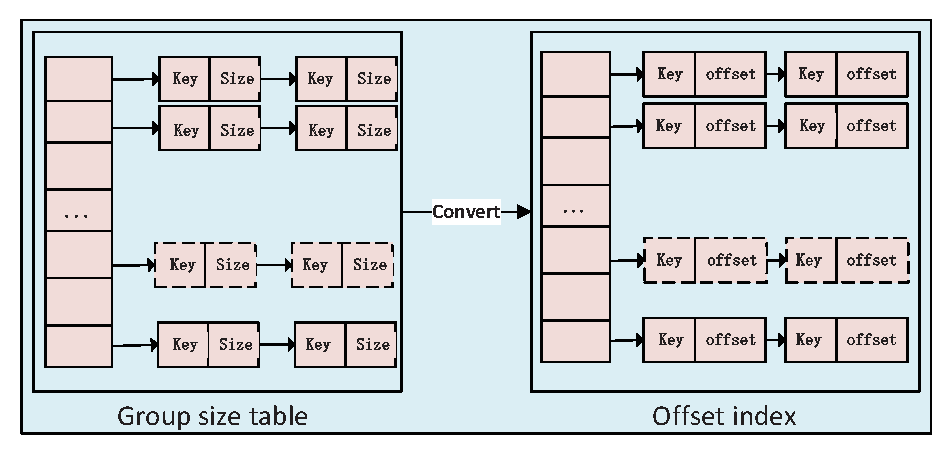
\includegraphics[width=.5\textwidth]{fig/convert}
\caption{The offset index generation.}
\label{fig:convert}
\end{figure}

Compared to the hash table in hash-based grouping methods, the offset index size is much less than the hash table where kv-pairs are stored, because the offset index only saves some integer --- the offsets---instead of storing kv-pairs. What's more, the big groups are processed separately in our algorithm, and the big groups are minority in the data sets, the space that the offset index occupies can be further reduce.
 
After constructing the offset index, the kv-pairs in big groups are written to the certain position in the result file depending on the corresponding offset. In the whole process, the big groups are not saved in memory in the whole group format, each kv-pair is read into memory and then written to the result file directly, only the offset index is always kept in memory, besides the necessay reading from and writing to the disk, there is no extra access to disk, so it can perform faster as shown in \ref{fig:paretoBig}. The profiling of this process shows that most of time is spent on seek operations during the file filling, this is mainly due to the fact that the writing of kv-pairs is not necessarily sequential, but filling the output files with big groups will lead to relatively large amount of sequential writes but less number of seeks.

\subsection{Phase 3: Partitioned Hash}

For a data set whose group sizes follow a power-law distribution, the majority of data set has been written to the result file after dealing with the big groups, the rest are small groups and the number of small groups are great than big groups, if we still employ indexing and filling method to group the kv-pairs in small groups, the size of offset index will increase a lot and may cause out-of-memory problem. In addition, the small group sizes vary over an small range, which can balanced division if we partition the small groups according to the available memory. In order to ensure the correctness of key grouping on small groups, the partition method we adopt is hashing, so we need to get the partition number, the partition number is determined by the available memory and the small groups number. 

For better analysis, we first define the following identifiers: the total size $T$ of data set, the current available memory $A$, the entry size $sizeof(entry)$ of the hash table used to grouping the small groups. In addition, the total size $S$ of small groups can be got after phase 1, the big group number $b$ can be obtained after phase 2. Combined with the ratio $r$ of big groups, the small group number $s$ is $b*(1-r)/r$. The space occupied when small groups are being processed is $S + sizeof(entry)*s$.
Because the actual hash table in small groups key grouping may be larger than the calculation, so we set an expansion factor $\alpha$ to expand the hash table size appropriately. So the partition number $P$ of small groups can be got like Formula \ref{eq:partition_num}. 
\begin{equation}\label{eq:partition_num}
    p = \dfrac{S + \alpha*sizeof(entry)*s}{A}
\end{equation}
For a kv-pair in a small groups, calculate the hash value $H_{key}$ first because the key may has various forms, and then hash the kv-pair to a partition depending on the partition id calculated by Formula \ref{eq:partition_hash}.
\begin{equation}\label{eq:partition_hash}
    id = H_{key} \%  p
\end{equation}  
Depending on the partition mode, the kv-pairs are hashed to different partitions, then the kv-pairs in small groups are grouped partition-by-partition by hash grouping method. Because the partition number is calculated roughly, the hash tables when dealing with several big parititions may be too large to be fit in memory, these great paritition will be divided into two parts and then be re-aggregated one-by-one, the repartition is an recursive process. Since the division is almost balanced, the repartition reduces a lot. Compared to the process of big groups, the partitioned hash grouping maintains the high performance of hashing grouping. Therefore, powerhash is an I/O efficient hash grouping approach with high performance in limited memory.  

\begin{algorithm}[ht]
    \caption{Power-Law Hash}
  \label{alg:group}
    \begin{algorithmic}[1]
    \Require  File \emph{F}, ratio \emph{r}, available memory \emph{A}, width \emph{w}, depth \emph{d}
    \Ensure result files $R$
    \State \emph{C:=} a two-dimensional array with width \emph{w} and depth \emph{d}
    \State \emph{H:=}\{\textbf{for} each \emph{i} \textbf{do} generate a hash function $h_i$, \emph{0 $\le$ i $\textless$d}\}    
    \State $key\_file :=$ a file of recording the key and value size
    \State initialize \emph{C = } \{\emph{C[$i$][$j$] = 0}, \emph{0 $\le$ i $\textless$d}, \emph{0 $\le$ j $\textless$ w} \}
    \For{each input $\langle key,value\rangle$ in \emph{F}}
    	\State write $\langle key,valuesize\rangle$ to the \emph{key\_file}
     	\For{ each $h_{i}() \in H $, \emph{0 $\le$ i $\textless$d} }
          \State \emph{C}[$i$][$h_{i}(key)$] += $sizeof(key) + sizeof(value)$
        \EndFor  
    \EndFor
    \State \emph{T:=} a group size table for the big groups
    \State calculate threshold \emph{t} between big groups and small groups.
    \For{each $\langle key,valuesize\rangle$ in \emph{key\_file}}
    	\State group size $f_{key}$ = \emph{min}(C[$i$][$h_{i}(key)$]), \emph{0 $\le$ i $\textless$d}
    	\If{ $f_{key} \textgreater$ \emph{t}}
    		\State insert the $\langle key,valuesize\rangle$ into \emph{T}    
    	\EndIf    	
    \EndFor
    \State calculte partition number \emph{p} depending on Fumula \ref{eq:partition_num}
    \State offset index $O:=Convert(T)$
    \State \emph{P:=} \{\textbf{for} each \emph{i} \textbf{do} generate a partition file $p_i$, \emph{0 $\le$ i $\textless$p}\}
    \For{ each input $\langle key,value\rangle$ in \emph{F}}
    	\If {there is a match in $O$ }
    		\State write the $\langle key,value\rangle$ into $R$
    		\State update the corresponding offset in $O$
    	\Else 
    		\State $id = H(key) \% p$
    		\State insert the $\langle key,value\rangle$ into $p_{id}$ 
    	\EndIf
    \EndFor
    \For{each $p_{id}$, \emph{0 $\le$ i $\textless$ p} }
		\State GroupBy($p_{id}$) in memory and Write to $R$
    \EndFor
    \State remove \emph{key\_file} and partition set \emph{P}
    \State output \emph{R}
    \end{algorithmic}
\end{algorithm}

\subsection{Algorithm analyse}
We summarize the whole process including the three phases in Algorithm \ref{alg:group}. The algorithm starts by creating a two-dimensional array with width \emph{w} and depth \emph{d} that is necessary to the CM sketch. Then each $\langle key, value\rangle$ pairs read from the input file \emph{F} is hashed to the CM sketch to calculate the rough size of each group. In order to avoid traversing the whole input file unnecessarily in phase 2, we use an intermediate file \emph{key\_file} to record the key and its corresponding value size in $\langle key, valuesize\rangle$ format during traversing the input file, i.e., we transform the original format $\langle key, value\rangle$ of the input data set into $\langle key, valuesize\rangle$ format, by which we can reduce the I/O cost and the computation of accurate group sizes in phase 2.

After counting the rough sizes, the threshold \emph{t} between the big groups and small groups is calculated depending on the CM sketch and the ratio $r$ of big groups(Line 12), we first sort one row of the two-dimensional array \emph{C} in descending order, the threshold \emph{t} is the ${d*r}^{th}$ element of the sorted row. While traversing the \emph{key\_file}, the $\langle key, valuesize\rangle$ belonging to big groups are insert to the group size table to calculate the accurate groug size like Formula \ref{eq:accurate_size}. The other $\langle key, valuesize\rangle$ pairs are accumulated to get the total size of small groups. We can get the group size table and other necessary factors after traversing the \emph{key\_file}, the partition number $p$ can be calculated like Formula \ref{eq:partition_num}, and offset index will be converted from the group size table.

The $Convert$ function converts the group size table to offset index (Line 22), in more details, traverses the elements in table $T$ from top to down and then accumulate the group sizes as the offset depending on the traversing order. The first entry of the table $T$(i.e. the first $\langle key, groupsize\rangle$) is the first group, so the initial offset of the entry equals to 0, it means that the first kv-pair mapped to the group will be stored in the beginning of the result file. Define the group size of the previous entry as $group_{pre}$, which means that the size of the previous group is $group_{pre}$. Define the initial offset of the previous group as ${off}_{pre}$. So the offset of current entry ${off}_{cur}$ equals to the sum of ${off}_{pre}$ and $group_{pre}$. After calculate the offset of each group, we will obtain an in-memory offset index which contains $\langle key,offset\rangle$ information. 

Finally, filling the result file phase needs another pass of the input file, the kv-pairs in big groups are written to the result file in terms of the offset index(see lines 22-25 in Algorithm \ref{alg:group}). For a kv-pair, get the offset ${off}_{key}$  by searching the offset index $O$, if there is a match in the index, it belongs to a big group and will be written to the ${off}^{th}_{key}$ bytes of the result file \emph{R} depending on the offset, if there is no match, it will be written to the corresponding partition in \emph{P}. With a kv-pair from input file having been output, the current offset of the corresponding group will increase the size of the kv-pair in bytes, which indicates the next kv-pair mapped to the same group will be stored in the ${({off}_{cur} + sizeof(\langle key,value\rangle ))}^{th}$ bytes of the file \emph{R}. It is the update operation in line 25 of Algorithm \ref{alg:group}.

After grouping the big groups successfully, the small group in each partitions stored in the disk are still unordered, these small group partitions are read into memory partition-by-partition and processed by the hash grouping, then these kv-pairs in small group partitions are appended to the result file \emph{R} after grouping(as shown 31-33 in algorithm \ref{alg:group}). 







%\input{disscussion}
\section{Experimental Evaluation}


This section presents the performance evaluation for PowerHash. We compare our work against existing typical grouping approaches, merge-sort \cite{dean2008mapreduce} and memory-constraint hash \cite{bartholomew2012mariadb}. For merge-sort, we downloaded the implementation from the official sites. There is no source code for memory-constraint hash available, so we implemented our own hash aggregation version following the pseudo code in SQL database \cite{HashAggregate15}. We used typical real data sets:  (a) the Higgs\footnote{http://snap.standford.edu/data/higgs-twitter.html} Twitter data set, providing the information about activity on Twitter during the discovery of Higgs-boson; (b) web-BerkStan \footnote{http://snap.stanford.edu/data/web-BerkStan.html} data set, a web graph containing 685,230 nodes and 7,600,595 edges;  (c) Google\footnote{http://snap.standford.edu/data/web-Google.txt.gz} data set, a web graph data set containing 875,713 nodes and 5,105,039 edges; and a simulation data set that obey a power-law distribution Pareto. Table 1 summarizes the data sets used.

\begin{table}[h]
  \caption{Data sets}
  \label{tab:dataset}
  \begin{tabular}{ccl}
    \toprule
    dataset &size & illustration\\
    \midrule
    Twitter & 180.4MB& Twitter social network statistics data\\
	web-BerkStan & 102.5MB& Berkely and Stanford web graph data\\
    Google & 97.2MB & Google web graph data\\
    Pareto & 575.4MB & Pareto distributed simulation data\\
    \bottomrule
  \end{tabular}
\end{table}

\begin{figure*}[htbp]
    \centering
  \subfloat[Overall performance on Twitter]{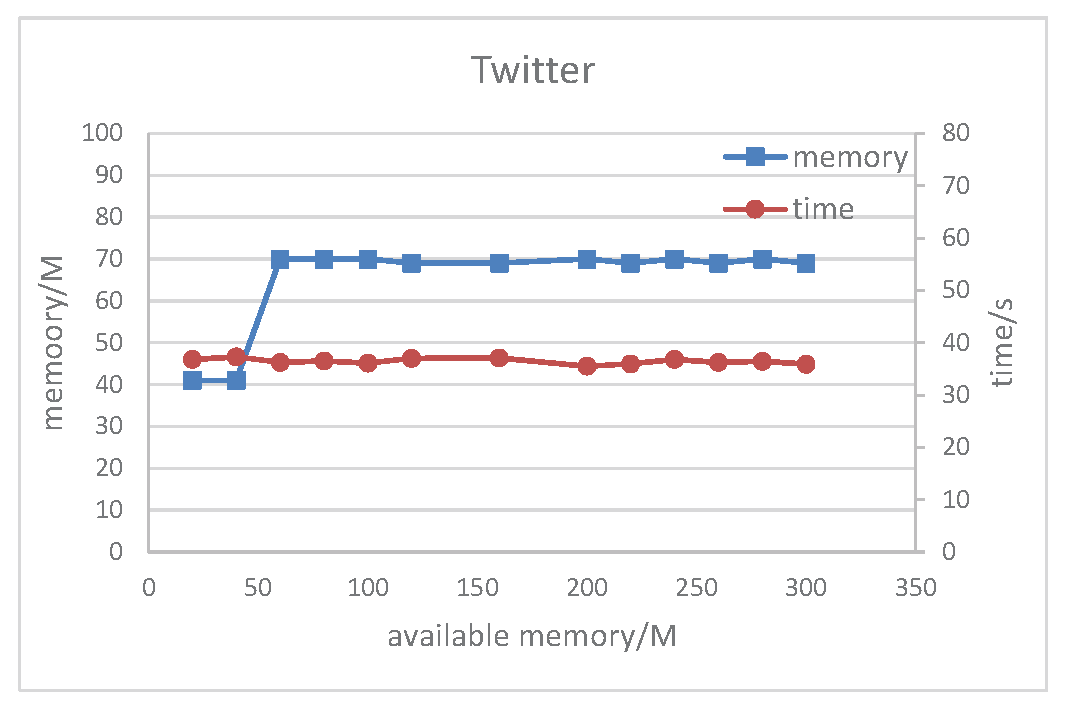
\includegraphics[width = 1.61in, height = 3.5cm]{fig/twitterMemTime.eps}\label{fig:twitterMemTime}}\ \
    \hspace{0.5pt}
  \subfloat[Overall performance on web-BerkStan]{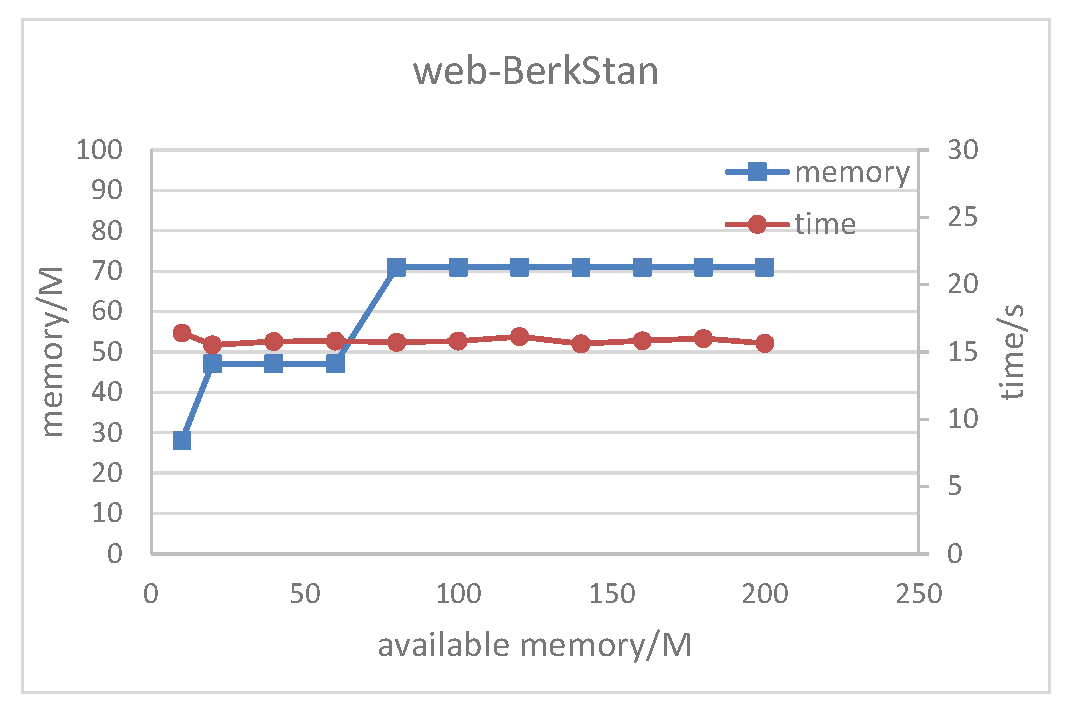
\includegraphics[width = 1.61in, height = 3.5cm]{fig/webMemTime.eps}\label{fig:webMemTime}}\ \
   \hspace{0.5pt}
  \subfloat[Overall performance on Google]{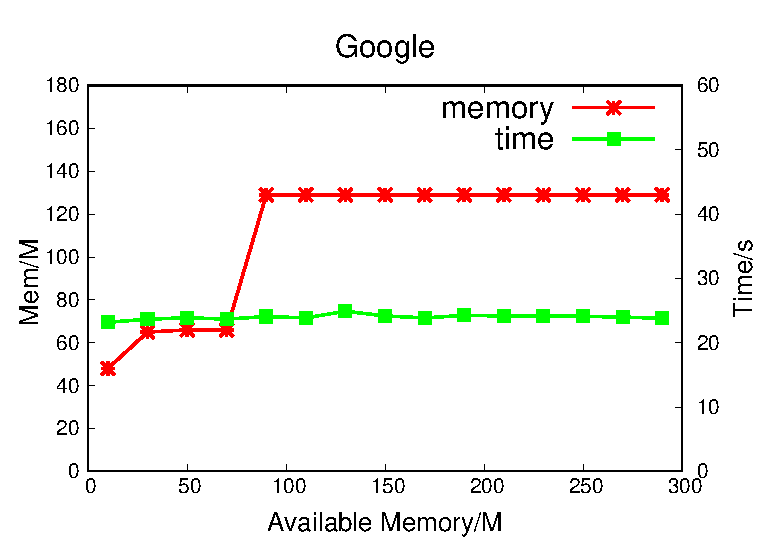
\includegraphics[width = 1.61in, height = 3.5cm]{fig/googleMemTime.eps}\label{fig:googleMemTime}}\ \
     \hspace{0.5pt}
  \subfloat[Overall performance on Pareto]{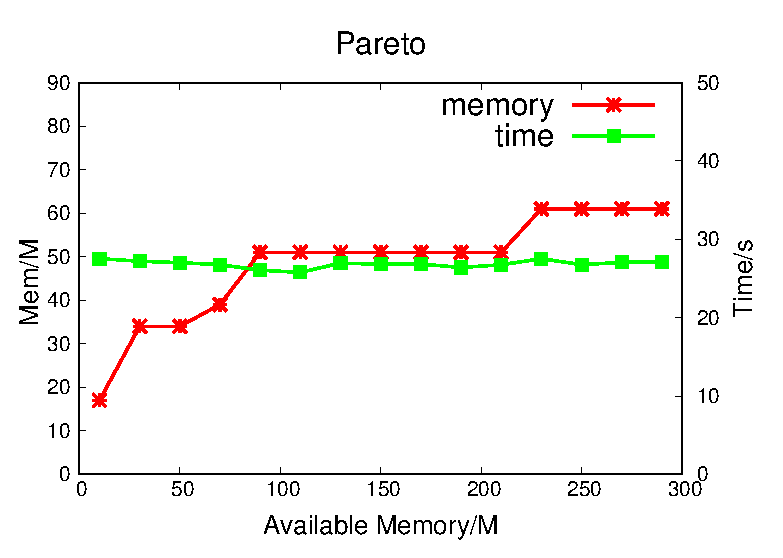
\includegraphics[width = 1.61in, height = 3.5cm]{fig/paretoMemTime.eps}\label{fig:paretoMemTime}}\ \ 
    \caption{Overall performance on various data sets.}
  \label{fig:overallPerformance} 
\end{figure*}

\begin{figure*}[htbp]
    \centering
  \subfloat[Performance comparison on Twitter]{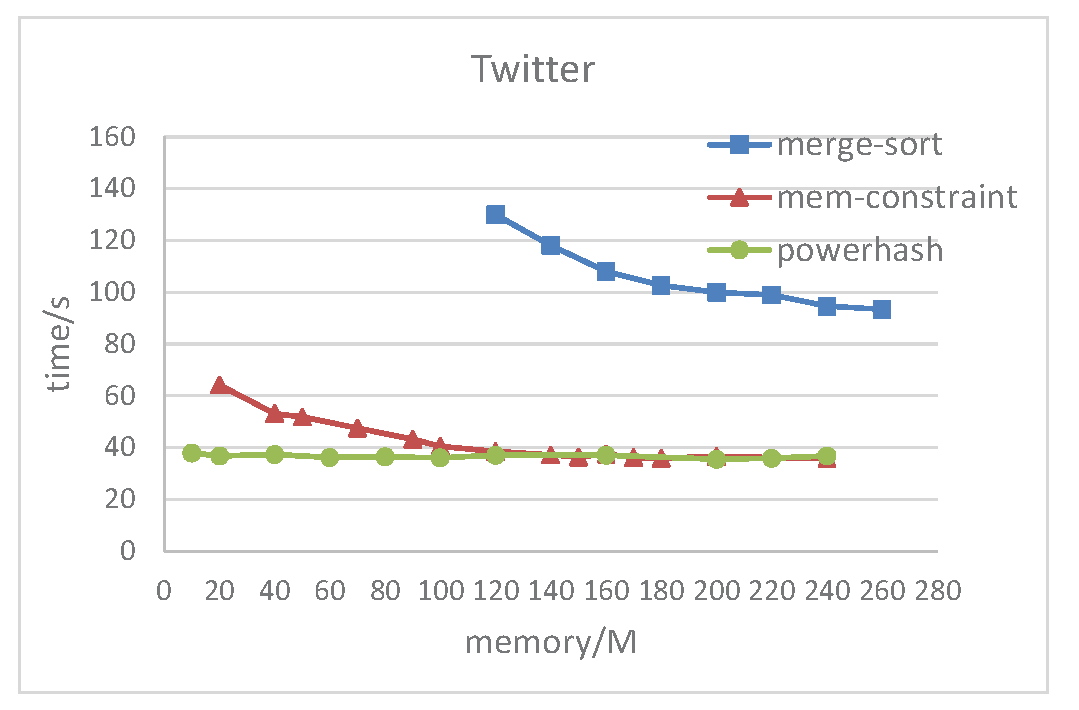
\includegraphics[width = 1.61in, height = 3.5cm]{fig/twitterComparison.eps}\label{fig:twitterComparison}}\ \
    \hspace{0.5pt}
  \subfloat[Performance comparison on web-BerkStan]{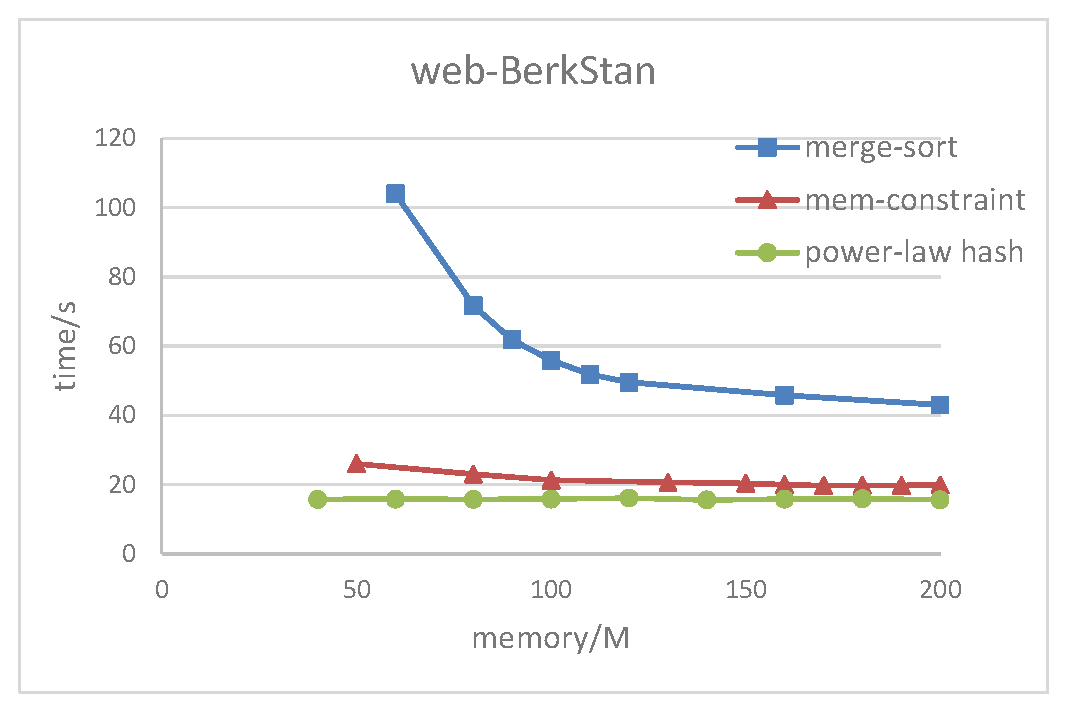
\includegraphics[width = 1.61in, height =3.5cm]{fig/webComparison.eps}\label{fig:webComparison}}\ \
   \hspace{0.5pt}
  \subfloat[Performance comparison on Google]{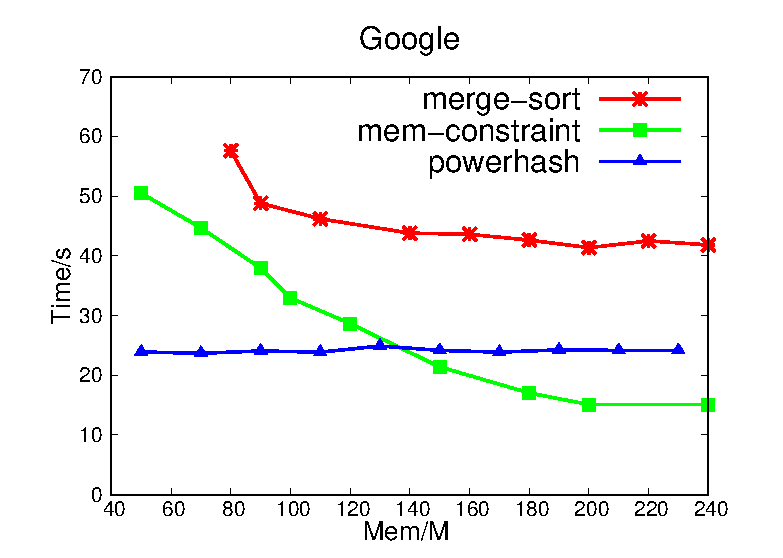
\includegraphics[width = 1.61in, height = 3.5cm]{fig/googleComparison.eps}\label{fig:googleComparison}}\ \
     \hspace{0.5pt}
  \subfloat[Performance comparison on Pareto]{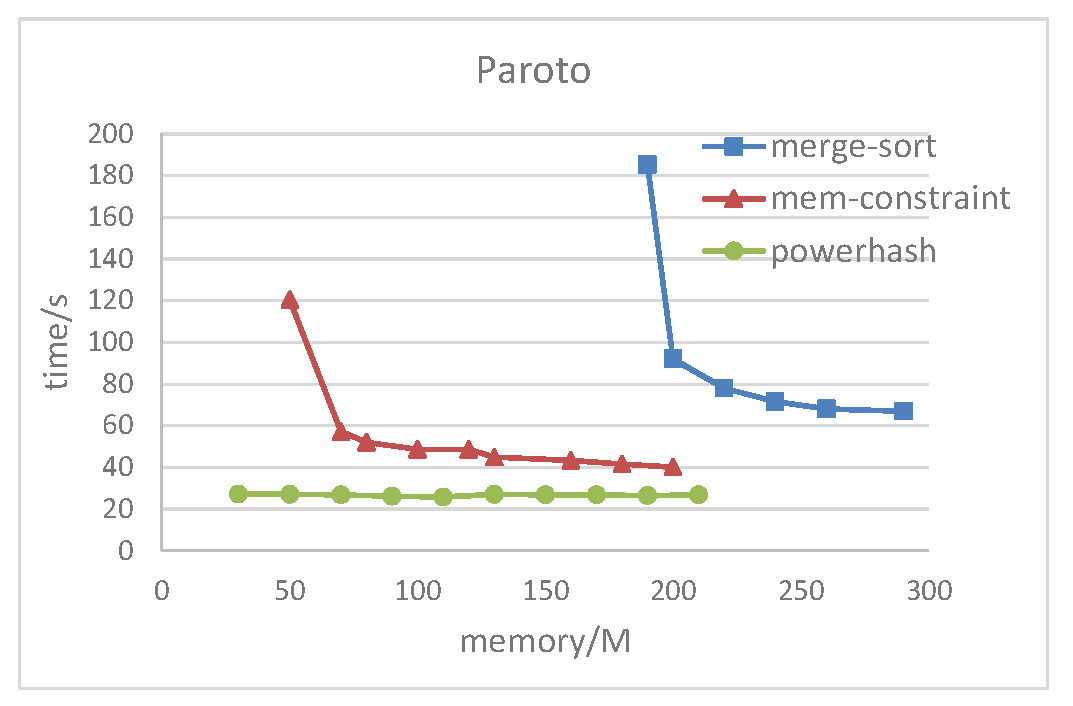
\includegraphics[width = 1.61in, height = 3.5cm]{fig/paretoComparison.eps}\label{fig:paretoComparison}}\ \ 
    \caption{Performance comparison on various data sets.}
  \label{fig:performanceComparison} 
\end{figure*}

All serial methods were implemented in C++, and compiled with g++ version 4.8.4 in Linux. The experiments were executed on a machine with two quad-core Intel CPUs at 2.67GHz and 32GB RAM.

\subsection{Overall Performance Evaluation}

The following experiments exhibits the overall performance of PowerHash and its performance comparison against merge-sort and memory-constraint hash. When executing PowerHash algorithm on various data sets, the most important parameter --- the ratio of big groups in these data sets is set as 0.2 depending the Pareto principle, the expansion factor proposed in section \ref{sec:hash} to ensure each small group partition can be processed in memory safely is set as 2. 

Figure \ref{fig:overallPerformance} exhibits the overall performance of PowerHash for different data sets as showed in Table \ref{tab:dataset}, it shows the real memory consumption and grouping time with the available memory varying. As the available memory varies, the grouping time is almost unchanged, even if the available memory is very small, the time cost in which case is nearly equal to the time cost with sufficient memory in Figure \ref{fig:twitterMemTime} \ref{fig:webMemTime} \ref{fig:googleMemTime} \ref{fig:paretoMemTime}. The reason for this phenomenon is that the available memory only influences the partition of small groups if the ratio of big groups is fixed, the grouping time of big groups keeps steady in theory no matter how much memory is available, and the grouping time of small groups is nearly the same when the partition numbers are not much different, so the whole time cost of PowerHash always keep stable. 

From Figure \ref{fig:overallPerformance}, we can also see that the memory consumption grows stage by stage and then stays stable. The statistical memory consumption in the line chart is the peak of memory usage in each experiment, according to the experimental results, these statistical peaks are always the space occupied by the hash table in small groups hash grouping process. So each jump of memory consumption represents a decrease of small groups partition number, the memory usage stays stable finally because there is enough memory to load the kv-pairs in small groups and the partition number decrease to 1. The minimal memory consumptions shown in Figure \ref{fig:overallPerformance} reveals the offset index size in indexing-filling, e.g., it is only 22MB as shown in Figure \ref{fig:twitterMemTime}, in other words, PowerHash can achieve its best performance with just about 22MB on Twitter. We can see that PowerHash can complete the key grouping operation with a little memory.
 
The next experiment investigates the scalability of our method. Figure \ref{fig:performanceComparison} shows the comparison of grouping time against merge-sort and memory-constraint hash with the memory available increasing, we list experimental results on different data sets. 
On the whole, our algorithm is almost distributed lower than other algorithms in Figure \ref{fig:performanceComparison}. Considering the extremely large input size, we would like to compare them with limited memory. When the memory is limited, our algorithm performs faster in the case of the same memory consumption, and it takes up less memory under the same time cost, the available memory smaller the advantage more obvious. For merge-sort and memory-constraint hash, the execution time continues to decline with the memory available increases constantly, when the memory is large enough to process kv-pairs in memory completely, the performance is no longer enhanced and grouping time stays stable, at that time memory-constraint hash degenerates into the pure hashing grouping method. The merge-sort needs more than 10 times memory and memory-constraint hash needs 5 times(i.e., 120MB) memory for Twitter to achieve the best state compared to our algorithm as shown on Figure \ref{fig:twitterComparison}, the experimental results on other data sets are similar with a little different multiples.

%When the available memory is not sufficient, the grouping time gap between the two method is larger. 
Compared to merge-sort and memory-constraint hash, the runtime gap is greatest at the beginning of the line charts, in which case the runtime of memory-constraint hash is at least 2 times than PowerHash with the same memory on the four data set, the multiples of runtime between merge-sort and PowerHash is greater. Then their gap continues to decline with the available memory increasing. Even if memory-constraint hash reaches the stable state, our algorithm runs at least 25\% faster on web-BerkStan and at least 60\% faster on Pareto as shown in Figure \ref{fig:webComparison} \ref{fig:paretoComparison}. Memory-constraint hash can achieve the same performance on Twitter and Google, its time consumption is also longer than PowerHash with the same memory before this point where they have the same runtime in Figure \ref{fig:twitterComparison} \ref{fig:googleComparison}, it can perform better than PowerHash on Google when the memory is sufficient. 
%With the same time cost, the memory usage of our algorithm is smallest in most cases, because the PowerHash runtime almost keeps stable, it can reach the best state by the smallest memory compared to the other two approaches.
   
We make the following analysis to this phenomenon: recall to section \ref{sec:related}, for merge-sort algorithm, there is unnecessary computational overhead in aggregating kv-pairs, the sort process reduces its performance, its time cost is always highest even if the memory is enough. For memory-constraint hash, one or more buckets will be selected to spill to disk when the memory used has reached the threshold, these spilled partitions will be read back to re-aggregate subsequently. The power-law distributions makes it more difficult to divide the work data into small uniform portions. For a larger bucket spilled to disk, subsequent reading back and re-aggregating may lead to recursively execute the algorithm many times when the memory is limited, the I/O overhead increases sharply. However, PowerHash deals with the big groups and small groups separately, the big groups processed by indexing and filling, and the small groups are processed via partitioned hash grouping approach, the two grouping method used to process the big groups and small groups can be carried out with limited memory and avoid repeat access to disk as introduced in section \ref{sec:hash}, so the performance of memory-constraint hash is slower than PowerHash with the same limited memory. If there is enough memory, all kv-pairs can be loaded in memory, memory-constraint hash degenerate into the pure hashing grouping method, its performance may be faster than PowerHash as shown in Figure \ref{fig:googleComparison}. Therefore, our algorithm is able to more efficient in limited memory compared to other algorithms.

\subsection{Parameters Evaluation}
\begin{figure*}[htbp]
    \centering
  \subfloat[Ratio test on Twitter]{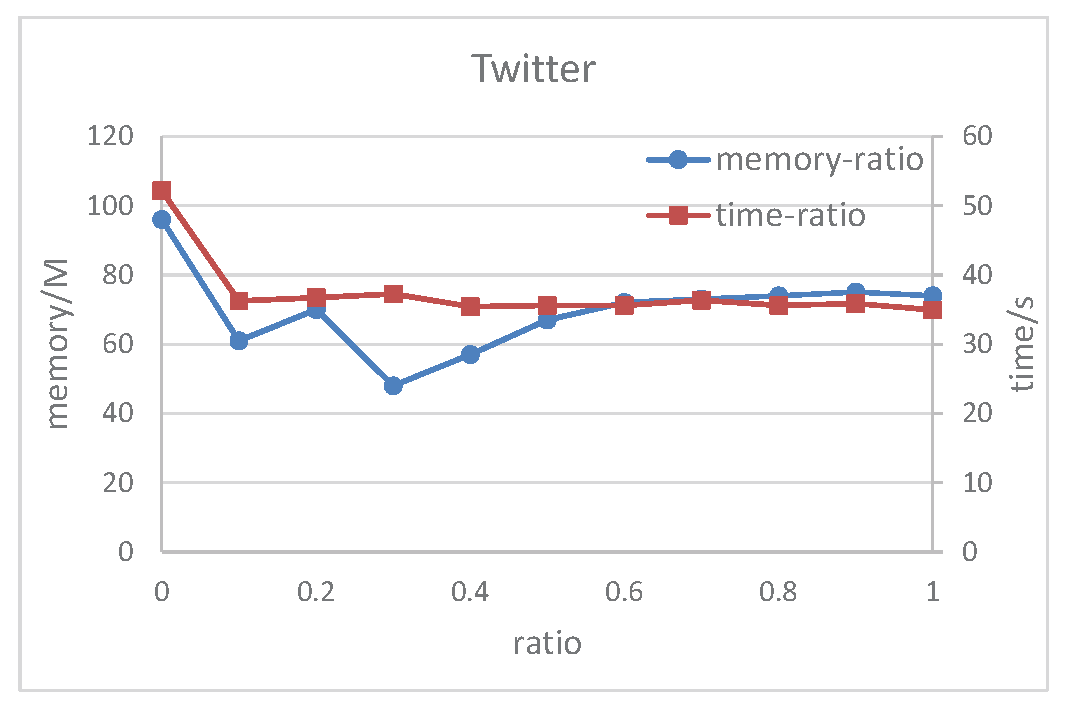
\includegraphics[width = 1.61in, height = 3.5cm]{fig/twitterRatio.eps}\label{fig:twitterRatio}}\ \
    \hspace{0.5pt}
  \subfloat[Ratio test on web-BerkStan]{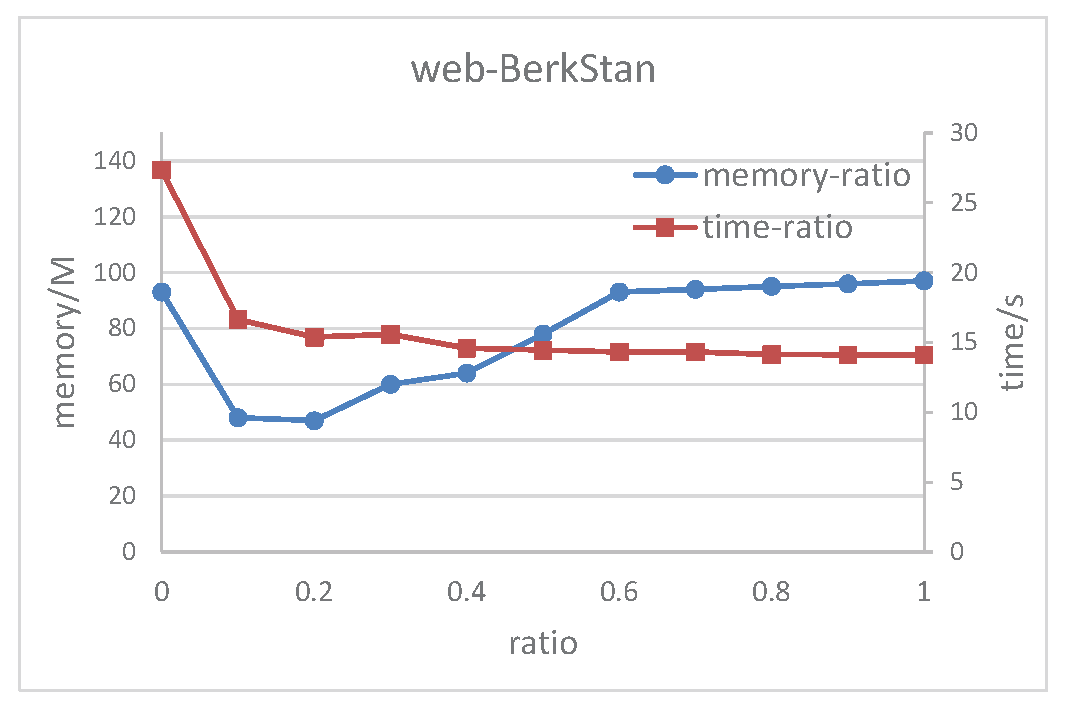
\includegraphics[width = 1.61in, height = 3.5cm]{fig/webRatio.eps}\label{fig:webRatio}}\ \
   \hspace{0.5pt}
  \subfloat[Ratio test on Google]{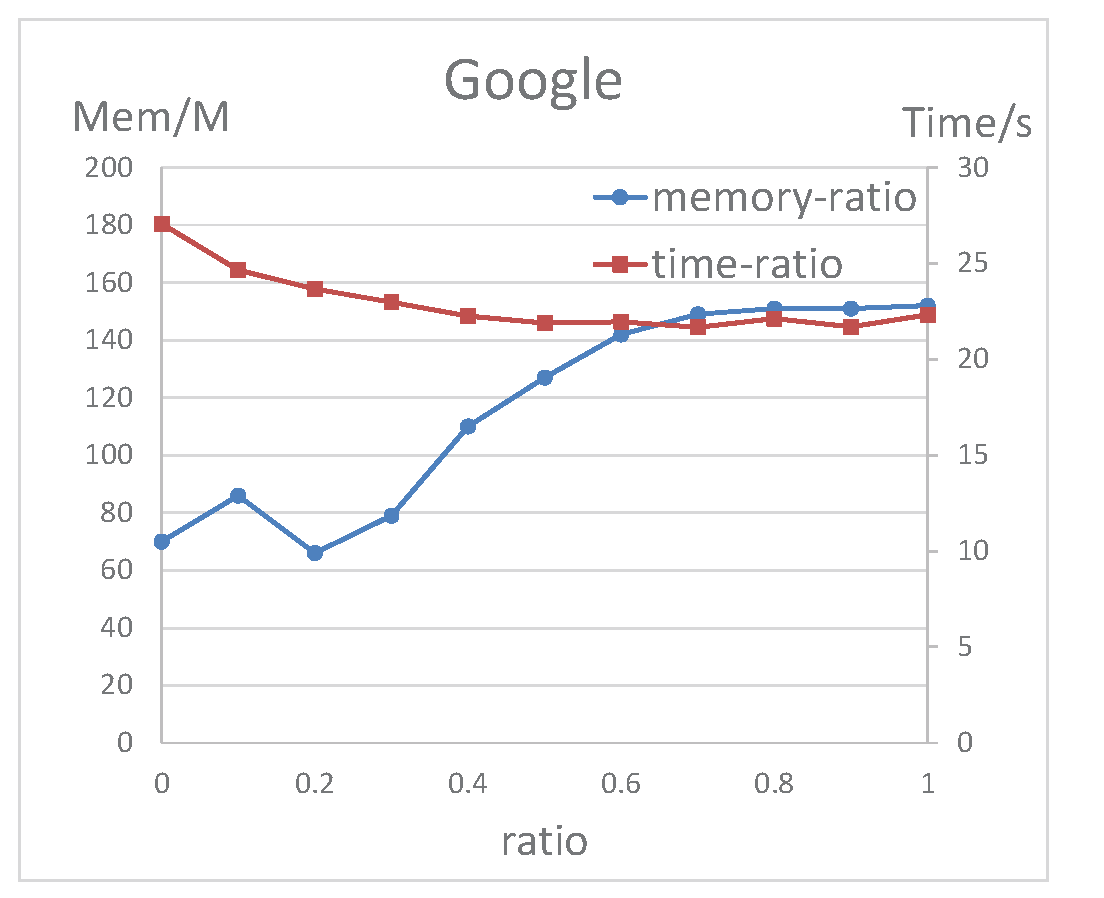
\includegraphics[width = 1.61in, height = 3.5cm]{fig/googleRatio.eps}\label{fig:googleRatio}}\ \
     \hspace{0.5pt}
  \subfloat[Ratio test on Pareto]{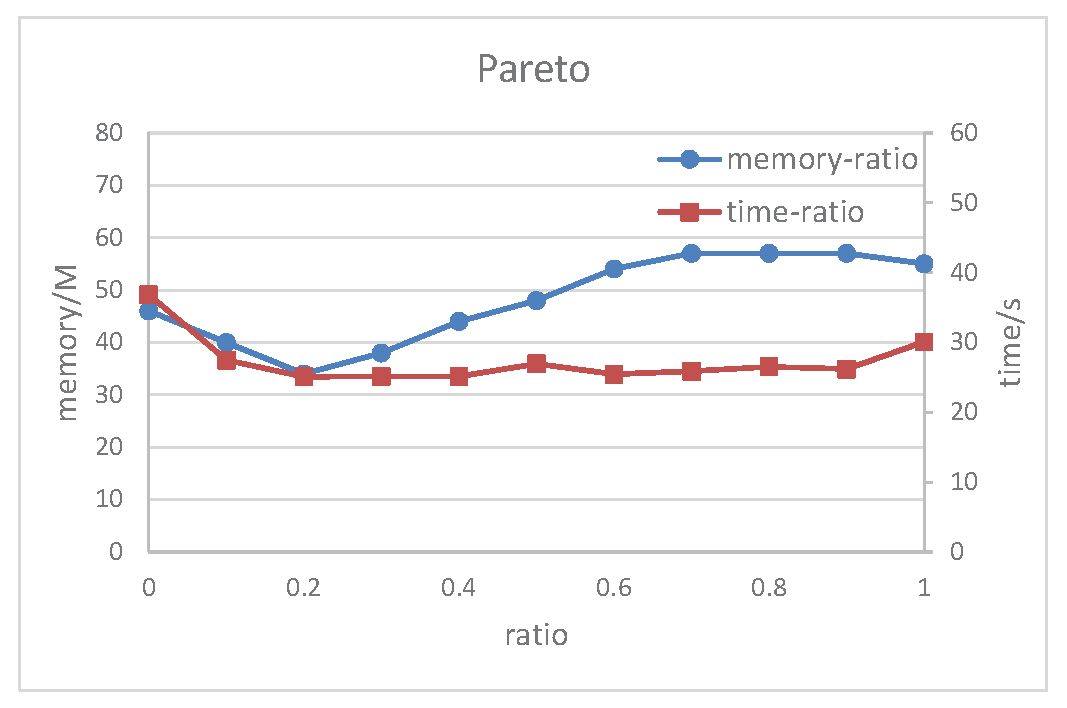
\includegraphics[width = 1.61in, height = 3.5cm]{fig/paretoRatio.eps}\label{fig:paretoRatio}}\ \ 
    \caption{Ratio test on various data sets.}
  \label{fig:ratio} 
\end{figure*}
In the work, we also evaluate the impact on different parameters of PowerHash. We have experimentally evaluated on various data sets in Table \ref{tab:dataset} and theoretically analyzed the effects of these parameters on the algorithm. Figure \ref{fig:ratio} shows the strong scalability results for the algorithm.

\textbf{The ratio of big groups}. The ratio of big groups is the most important parameter in PowerHash, it determines the division between big groups and small groups. Compared with the real ratio of big groups in the data sets, a smaller ratio may lead to the unbalance of small group partitions because some big groups are judged as small groups, and then cause the redivision of small groups; a bigger ratio may result in a great offset index of big groups and then causes the waste of memory, so the selection of ratio is important. As shown in Figure \ref{fig:ratio}, the ratio is set from 0 to 1, the available memory is fixed and set as 50MB, PowerHash becomes the partitioned hash method when the ratio is 0, it turns to the indexing and filling method when the ratio is 1, their memory usage is much larger than 50MB in both cases and the out-of-memory problem will occur. With the ratio varying, the execution time decreases and then stays stable, the memory usage continues to decline and then continues to increase, the point with least memory usage represents the offset index size and small group partition sizes are the most suitable, and the memory usage is under 50MB in this case, i.e., the algorithm can be executed in memory smoothly without out-of-memory problem. In Figure \ref{fig:webRatio} \ref{fig:googleRatio} \ref{fig:paretoRatio}, the memory usage is lowest when the ratio is 0.2, this phenomenon satisfies the Pareto principle. In Figure \ref{fig:twitterRatio}, our algorithm performs best when the ratio is 0.3. The experiment on these data sets can reflect the most appropriate ratio of big groups is the value around 0.2.
 
\textbf{The parameters of CM sketch}. The next experiment shows the effect of the CM sketch parameters. Recall from Distinction phase in section \ref{sec:hash} that the CM sketch are employed to reflect the distributions of group sizes, we sort a row of the CM sketch and then obtain the threshold between big group sizes and small group sizes according to the big groups ratio, then divide the big groups and small groups based on their rough sizes, so the width and depth of CM sketch can influence the judgement of big groups and small groups. According to the CM sketch introduction in section \ref{sec:related}: if the error of group sizes is within a factor of $ \varepsilon $ with probability $ \delta$, the depth is $\lceil ln(1/\delta)\rceil $, the width is $\lceil e/\varepsilon\rceil $, the depth can be set easily. The width of CM sketch determines the accuracy of threshold, it directly affects the division between big groups and small groups in Distinction phase. Figure 7 shows the memory usage and time cost on different data sets with the width varying.
\begin{figure}[htbp]
	\label{fig: CMPara}
    \subfloat[Runtime with different width]{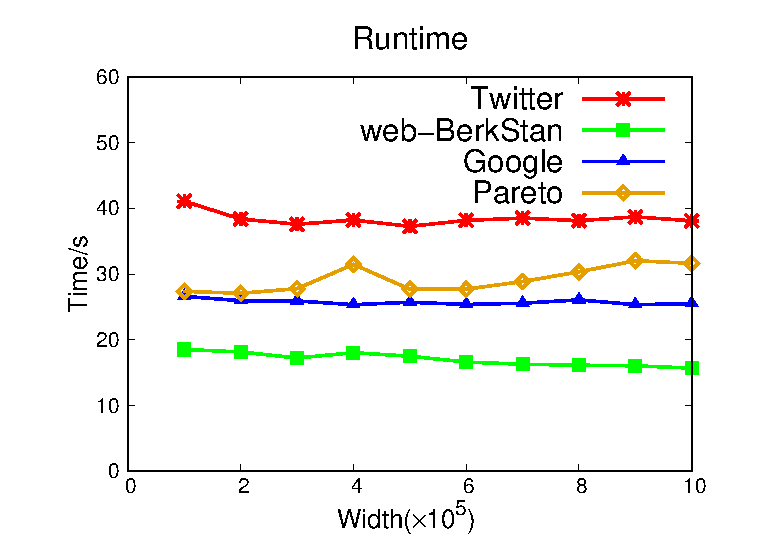
\includegraphics[width = 1.68in, height = 3.5cm]{fig/CMTime.eps}\label{fig:CMTime}}
       \hspace{0.23cm}
    \subfloat[Memory usage with different width]{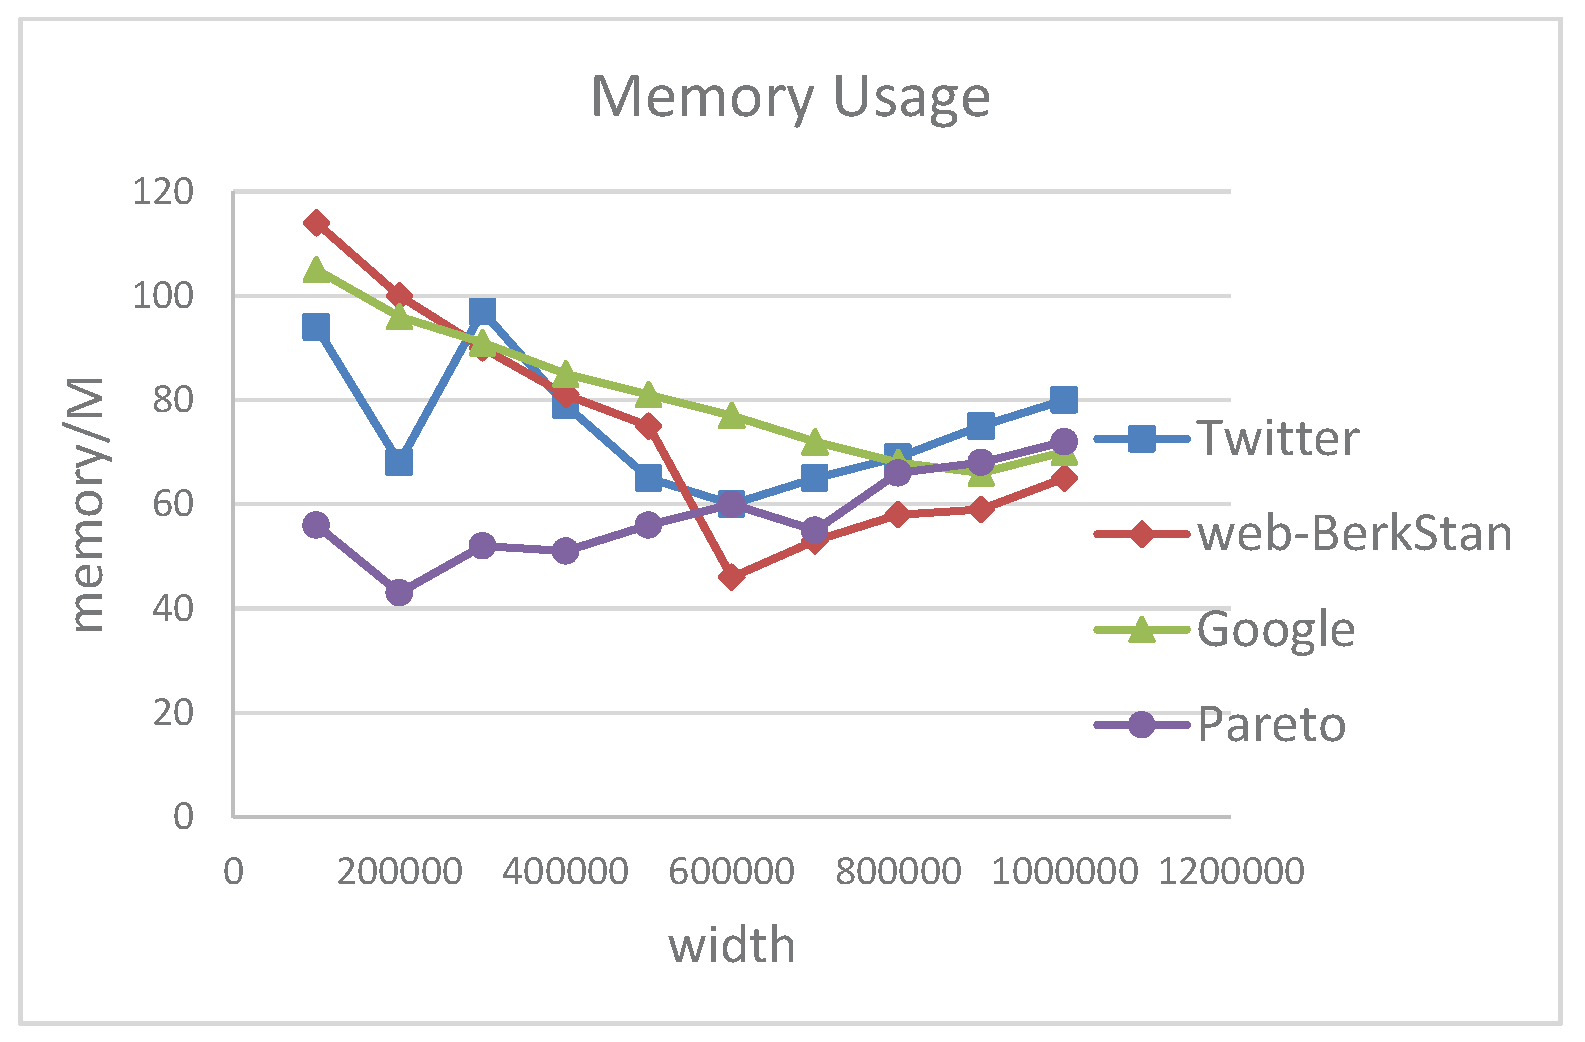
\includegraphics[width =1.68in, height = 3.5cm]{fig/CMMem.eps}\label{fig:CMMem}}\\    
	\caption{Runtime and memory usage with different width of the CM sketch.}	
	
\end{figure}

The runtime on each data set is almost steady as shown in Figure \ref{fig:CMTime}, the memory usage is influenced by the width of CM sketch as shown in Figure \ref{fig:CMMem}, it is appropriate to set the width from 200000 to 800000 with little memory waste.   

\subsection{Phase Evaluation}
In this subsection, we discuss the impact and interrelated factor on Distinction phase, Big groups grouping phase, Small groups grouping phase. Figure 8 shows the time percentage and memory consumption on the three phases. 

\begin{figure}[htbp]	
	\label{fig: PhaseEvaluation}
    \subfloat[Time percentage of each phase]{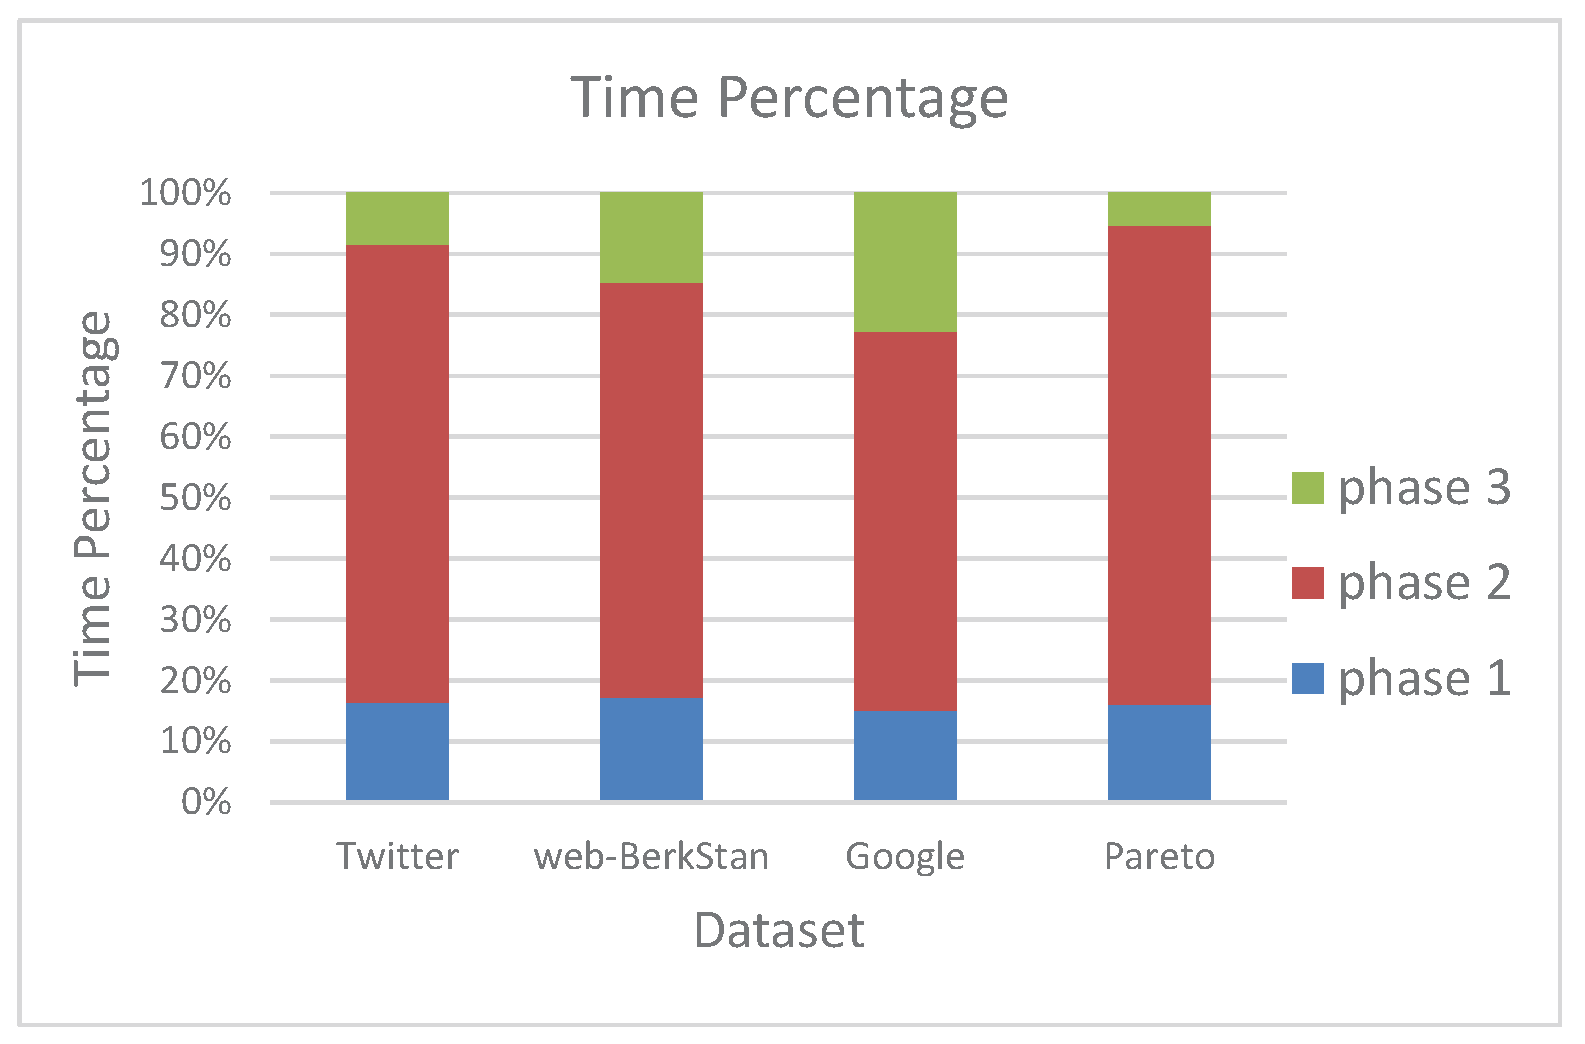
\includegraphics[width = 1.68in, height = 3.5cm]{fig/TimePercentage.eps}\label{fig:TimePercentage}}
    \hspace{0.23cm}
    \subfloat[Memory usage of each phase]{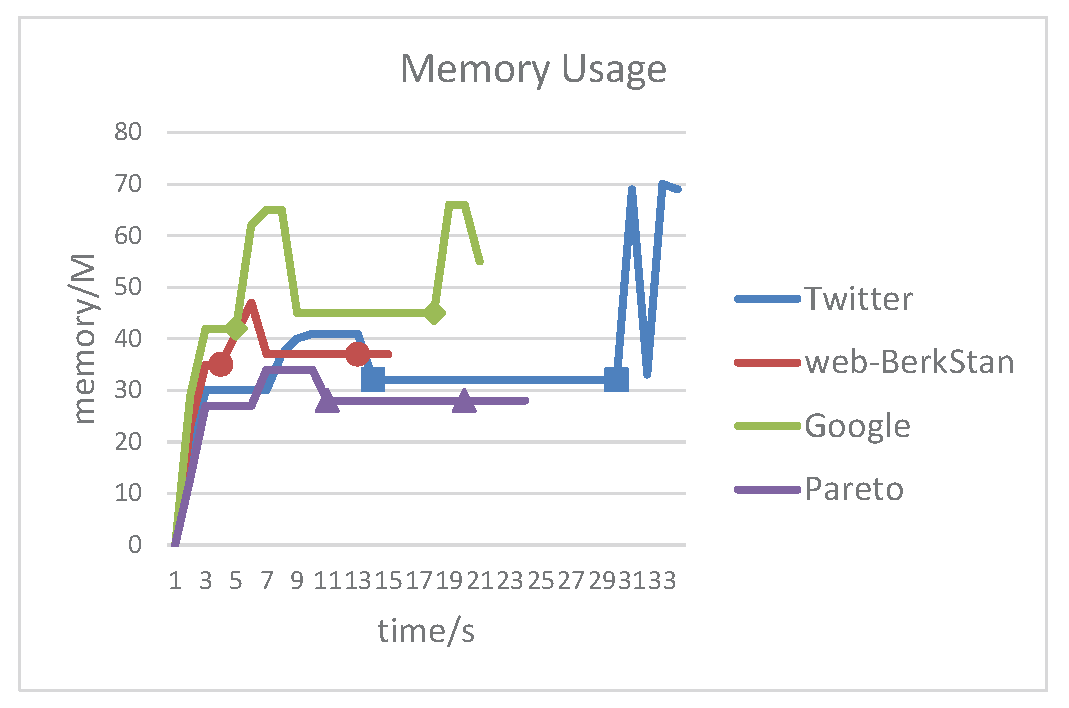
\includegraphics[width =1.68in, height = 3.5cm]{fig/MemPhase.eps}\label{fig:MemPhase}}\\    
	\caption{Runtime and memory usage comparison between each phase.}
		
\end{figure}

Figure \ref{fig:TimePercentage} shows the time percentage of the three phases on different data sets. We can notice that the time percentage of Distinction phase is close to 15\%, i.e., the preparation time of key grouping operation occupies 15\% of the total time. The Big groups grouping phase takes up most of the total time, the Small groups grouping phase groups the small groups with little time cost. This phenomenon satisfies expected result, the third phase is finished in memory so its time cost is small, the majority of the data set is processed in the second phase, and lots of time is spent on seeking operations, so its time percentage is highest.

We also compare the memory usage for the three phases on various data sets as depicted in Figure \ref{fig:MemPhase}. The mark point on each line separates the three phases. The memory usage continues to increase and keeps stable in the first phase, the memory usage in stale state is the size of CM sketch. Then the memory usage increases over time gradually in the second phase, its growth represents the generation of offset index, it decreases after the memory occupied by the CM sketch being released. In the third phase, the memory usage is also steady because the partition of small groups is balanced and each hash table in grouping process is almost the same.




\section{Conclusions}

Grouping key value pairs are essential for many practical applications that include MapReduce, SQL Hash Group By, etc. The volume of such data increases rapidly, therefore, it is essential to improve fast key value grouping methods. In this paper we proposed PowerHash, a method that supports very long records, large data sets and works efficiently even if the memory is very limited and is easily implemented. Extensive experimental evaluation with real data sets whose group sizes follow the power-law distributions revealed that our method is much more efficient than existing ones in terms of speed and computational resources, it can reduce the repeat access to disk caused by the distribution unbalance effectively when grouping these data sets. When the available is limited, our algorithm runs faster than merge-sort and memory-constraint hash with the same memory. The merge-sort and memory-constraint hash need several times memory to achieve the best state compared to our algorithm, it can help us save a large amount of memory when executing key grouping operation. This work is part of a large project that aims to develop an engine for grouping and processing of massive data. We are currently working on scaling our method to the distributed computing framework. As we know, stand-alone aggregating key value pairs of different groups is applied to both map phase and reduce phase in MapReduce independently. So PowerHash is easily parallelizable. We are also focusing on the parallel processing various types of grouping using the PowerHash.




\begin{bibliographystyle}{IEEEtran}
\bibliography{bibfile}
\end{bibliographystyle}

\end{document}


